% =============================================================================
% AI-Powered Sign Language Recognition System
% A Comparative Study of Image-Based and Landmark-Based Approaches
%
% Author: Yusuf Kenan Akgun (20210702010)
% Yeditepe University, Department of Computer Engineering
% CSE492 - Engineering Project, 2026
%
% Compile with:  pdflatex main && biber main && pdflatex main && pdflatex main
% (or: latexmk -pdf main.tex)
% =============================================================================

\documentclass[12pt,a4paper,oneside]{report}

% =============================================================================
% Preamble - tüm paket importları, sayfa düzeni, font, başlık stilleri
% =============================================================================

% --- Encoding & language --------------------------------------------------
\usepackage[T1]{fontenc}
\usepackage[utf8]{inputenc}
\usepackage[english]{babel}

% --- Page geometry --------------------------------------------------------
% A4, 3.5 cm sol cilt payı, 2.5 cm diğer kenarlar
\usepackage[
  a4paper,
  top=2.5cm,
  bottom=2.5cm,
  left=3.5cm,
  right=2.5cm,
  headheight=14.5pt,
  headsep=0.7cm,
  footskip=1.0cm,
]{geometry}

% --- Math packages (must load BEFORE newtxmath to avoid \Bbbk clash) ------
\usepackage{amsmath, amssymb, amsthm}

% --- Fonts (Times New Roman benzeri) --------------------------------------
\usepackage{newtxtext}     % gövde metni
\usepackage{newtxmath}     % matematik fontu (uyumlu, amssymb'den sonra)
\usepackage{microtype}     % blok hizalamada profesyonel görünüm

% --- Line spacing ---------------------------------------------------------
\usepackage{setspace}
\onehalfspacing            % 1.5 satır aralığı (akademik tez standardı)

% --- Paragraph style ------------------------------------------------------
\setlength{\parindent}{1.27cm}   % ilk satır girintisi (Word default)
\setlength{\parskip}{0pt}        % paragraflar arası ekstra boşluk yok

% --- Units & symbols ------------------------------------------------------
\usepackage{siunitx}
\sisetup{
  detect-all,
  group-separator={,},
  group-minimum-digits=4,
}

% --- Graphics & figures ---------------------------------------------------
\usepackage{graphicx}
\graphicspath{{figures/}}
\usepackage{float}         % [H] placement
\usepackage{subcaption}    % alt-figürler
\usepackage{rotating}      % sidewaysfigure (geniş diyagramlar için)

% --- Tables ---------------------------------------------------------------
\usepackage{booktabs}      % toprule/midrule/bottomrule
\usepackage{array}
\usepackage{multirow}
\usepackage{tabularx}
\usepackage{longtable}     % sayfa kıran tablolar

% --- Captions -------------------------------------------------------------
\usepackage[
  font=small,
  labelfont=bf,
  labelsep=period,
  justification=centering,
]{caption}

% --- Colors & code listings -----------------------------------------------
\usepackage{xcolor}
\definecolor{codegray}{rgb}{0.95,0.95,0.95}
\definecolor{codeblue}{rgb}{0.0,0.2,0.6}
\definecolor{codegreen}{rgb}{0.0,0.5,0.0}

% --- Algorithms (pseudo-code) ---------------------------------------------
\usepackage{algorithm}
\usepackage{algpseudocode}

% --- Headers & footers ----------------------------------------------------
\usepackage{fancyhdr}
\pagestyle{fancy}
\fancyhf{}
\fancyhead[L]{\nouppercase{\leftmark}}
\fancyfoot[C]{\thepage}
\renewcommand{\headrulewidth}{0.4pt}
\renewcommand{\footrulewidth}{0pt}

% Chapter ilk sayfasında "plain" stil, sadece sayfa numarası
\fancypagestyle{plain}{%
  \fancyhf{}
  \fancyfoot[C]{\thepage}
  \renewcommand{\headrulewidth}{0pt}
}

% --- Chapter title style (sade, profesyonel) ------------------------------
\usepackage{titlesec}
\titleformat{\chapter}[display]
  {\normalfont\Large\bfseries}
  {\chaptertitlename\ \thechapter}
  {12pt}
  {\LARGE}
\titlespacing*{\chapter}{0pt}{-20pt}{20pt}

% --- TOC / LOF / LOT formatting -------------------------------------------
\usepackage{tocloft}
\renewcommand{\cftchapfont}{\bfseries}
\renewcommand{\cftchappagefont}{\bfseries}
\setlength{\cftbeforechapskip}{6pt}
% LoF/LoT girişleri arası boşluk: çok cümleli caption'ların ikinci sayfaya
% taşmamasını sağlayacak kadar sıkı, fakat sayfa altında geniş boşluk
% bırakmayacak kadar ferah.
\setlength{\cftbeforefigskip}{8pt}
\setlength{\cftbeforetabskip}{8pt}

% --- Bibliography (IEEE style) --------------------------------------------
\usepackage{csquotes}
\usepackage[
  backend=biber,
  style=ieee,
  sorting=none,
  maxbibnames=99,
]{biblatex}
\addbibresource{references.bib}
\setlength{\bibitemsep}{6pt}
\AtBeginBibliography{\normalsize}

% --- Hyperlinks (en sonda olmalı) -----------------------------------------
\usepackage[
  colorlinks=true,
  linkcolor=black,
  citecolor=black,
  urlcolor=blue!60!black,
  pdfborder={0 0 0},
  bookmarksnumbered=true,
]{hyperref}
\usepackage[capitalize,noabbrev]{cleveref}

% --- Custom commands ------------------------------------------------------
\newcommand{\todo}[1]{\textcolor{red}{\textbf{[TODO: #1]}}}
\newcommand{\thesistitle}{On-Device American Sign Language Recognition: A Comparative Study of Image- and Landmark-Based Approaches for Mobile Deployment}
\newcommand{\thesisauthor}{Yusuf Kenan Akg\"un}
\newcommand{\thesisid}{20210702010}
\newcommand{\thesisadvisor}{Bet\"ul Arslan}
\newcommand{\thesisyear}{2026}
\newcommand{\thesisdepartment}{Department of Computer Engineering}
\newcommand{\thesisuniversity}{Yeditepe University}
\newcommand{\thesisfaculty}{Faculty of Engineering}


\begin{document}

% --- Front matter (Roman page numbers) ------------------------------------
\pagenumbering{roman}

% =============================================================================
% Title page - Yeditepe University CSE492 thesis cover
% Layout mirrors the Yeditepe sample (ornek-tez/Halil_Ertan_20220702109.pdf):
% title (uppercase, large, bold) at top; "by" + author + student ID centered
% mid-upper; "Engineering Project Report" mid-lower; university block at the
% bottom. The advisor is shown on the approval page, not on the cover.
% =============================================================================
\begin{titlepage}
  \thispagestyle{empty}
  \begin{center}
    \vspace*{1cm}

    {\LARGE \bfseries \MakeUppercase{\thesistitle} \par}

    \vspace{4cm}

    {\large \textbf{by}}\\[0.4cm]
    {\large \textbf{\thesisauthor}}\\[0.2cm]
    {\large \textbf{\thesisid}}

    \vspace{4cm}

    {\large \textbf{Engineering Project Report}}

    \vfill

    {\large \textbf{\thesisuniversity}}\\[0.15cm]
    {\large \textbf{\thesisfaculty}}\\[0.15cm]
    {\large \textbf{\thesisdepartment}}\\[0.15cm]
    {\large \textbf{\thesisyear}}

    \vspace{0.5cm}
  \end{center}
\end{titlepage}

% titlepage ortamı sayacı 1'e resetler; kapağı "i" sayıp boş sayfayı "ii",
% onay sayfasını "iii" olarak numaralandırmak için sayacı 2'ye alıyoruz.
\setcounter{page}{2}

% Boş sayfa (kapakla onay sayfası arasında, ciltleme için) — numara gizli
\thispagestyle{empty}
\null
\clearpage

% =============================================================================
% Approval (signature) page - mirrors Yeditepe sample
% (ornek-tez/Halil_Ertan_20220702109.pdf): title at top (cover style),
% "APPROVED BY:" left-aligned; signature block centered with [name | signature]
% rows; "DATE OF APPROVAL:" left-aligned at the bottom.
% =============================================================================
\thispagestyle{plain}
\begin{center}
  \vspace*{1cm}

  {\LARGE \bfseries \MakeUppercase{\thesistitle} \par}
\end{center}

\vspace{3cm}

\noindent{\Large \bfseries APPROVED BY:}

\vspace{1.5cm}

\begin{center}
  {\large
  \begin{tabular}{l@{\hspace{1.5cm}}l}
    \thesisadvisor\ \textit{(Supervisor)} & \makebox[3cm]{\dotfill} \\[1cm]
    \makebox[6cm]{\dotfill}               & \makebox[3cm]{\dotfill} \\[1cm]
    \makebox[6cm]{\dotfill}               & \makebox[3cm]{\dotfill} \\
  \end{tabular}
  }
\end{center}

\vfill

\noindent{\Large \bfseries DATE OF APPROVAL:}\ \ {\Large \makebox[1.2cm]{\dotfill}/\makebox[1.2cm]{\dotfill}/\thesisyear}

\vspace{1cm}

\clearpage


\chapter*{Acknowledgements}
\addcontentsline{toc}{chapter}{Acknowledgements}

\todo{Write acknowledgements paragraph.}

\clearpage

\chapter*{Abstract}
\addcontentsline{toc}{chapter}{Abstract}

\begin{spacing}{1.4}
This thesis presents an end-to-end American Sign Language (ASL)
recognition system that runs entirely on a consumer Android phone.
Two complementary tasks are addressed: fingerspelling recognition
over the 29 classes of the ASL Alphabet dataset, and word-level
recognition over the 100-class WLASL-100 vocabulary. For the letter
task, two classifiers are trained and compared: an EfficientNet-B0
that consumes raw image crops and a compact multi-layer perceptron
over 21 MediaPipe hand landmarks. On the single-signer ASL Alphabet
test split they reach \SI{100}{\percent} and \SI{99.38}{\percent}
Top-1 respectively, read as a pipeline sanity check rather than
capability claims; the landmark model ships in a \SI{0.24}{MB}
checkpoint. A single-user on-device manual evaluation under
realistic camera conditions inverts the offline ranking on the
budget phone (landmark MLP \SI{100}{\percent}, image network
\SI{92.9}{\percent}), motivating the landmark variant as the
deployment default for the letter task. For the word task, a
bidirectional LSTM is trained on a two-handed 128-dimensional
landmark feature stream extracted from a yt-dlp-recovered WLASL-100
corpus (\num{1465} clips, a \SI{44}{\percent} increase over the
\num{1013}-video Kaggle baseline). A five-seed logit-averaging
ensemble reaches \SI{56.22}{\percent} Top-1 and
\SI{81.09}{\percent} Top-5 on the WLASL-100 test partition under
the canonical person-mixed split, clearing the \SI{40}{\percent}
Top-1 acceptance bar adopted for this thesis by sixteen percentage
points. Because the protocol is person-mixed by design, this
offline figure is positioned as a literature-comparable benchmark
point under that protocol rather than as a signer-independent
generalization estimate. A nine-step forward-additive ablation
decomposes the gain from a \SI{20}{\percent} baseline to the
\SI{60.08}{\percent} final validation accuracy into three pillars
of comparable weight: data engineering, the extraction pipeline,
and training-recipe refinements. All four classifiers are exported
to TensorFlow Lite and deployed in an Android application built
around CameraX and MediaPipe Hands. On-device throughput, latency,
and the OOD accuracy gap are characterised on a budget
(TECNO SPARK 20C) and a flagship (Xiaomi 15T Pro); word accuracy
is flagship-only because entry-level ensemble latency is too high
for interactive use. The evaluation produces a device-conditional
model-selection guideline.
\end{spacing}

\clearpage

\chapter*{\"Ozet}
\addcontentsline{toc}{chapter}{\"Ozet}

Bu tez, t\"um\"uyle bir t\"uketici Android telefon \"uzerinde
\c{c}al{\i}\c{s}an u\c{c}tan uca bir Amerikan \.I\c{s}aret Dili
(ASL) tan{\i}ma sistemi sunmaktad{\i}r. \.Iki t\"umleyici g\"orev
ele al{\i}n{\i}r: ASL Alphabet veri k\"umesinin 29 s{\i}n{\i}f{\i}
\"uzerinden parmak ile harf tan{\i}ma ve WLASL-100 veri
k\"umesinin 100 kelimelik s\"ozda\u{g}arc{\i}\u{g}{\i} \"uzerinden
kelime tan{\i}ma. Harf g\"orevi i\c{c}in iki s{\i}n{\i}fland{\i}r{\i}c{\i}
e\u{g}itilip kar\c{s}{\i}la\c{s}t{\i}r{\i}lm{\i}\c{s}t{\i}r: ham
g\"or\"unt\"u kesitlerini girdi olarak alan bir EfficientNet-B0 ve
MediaPipe ile \c{c}{\i}kar{\i}lan 21 el i\c{s}aret noktas{\i}n{\i}
girdi olarak alan, kompakt bir \c{c}ok-katmanl{\i} alg{\i}lay{\i}c{\i}
(MLP). Ayr{\i}lm{\i}\c{s} test b\"ol\"um\"unde s{\i}ras{\i}yla
\%100 ve \%99{,}38 Top-1 do\u{g}rulu\u{g}una ula\c{s}m{\i}\c{s}lar,
landmark tabanl{\i} modelin a\u{g}{\i}rl{\i}\u{g}{\i} 0{,}24 MB
boyutunda kalm{\i}\c{s}t{\i}r. Kelime g\"orevi i\c{c}in
\c{c}ift-elli 128 boyutlu landmark \"oznitelik dizisi \"uzerine
\c{c}ift-y\"onl\"u bir LSTM e\u{g}itilmi\c{s}; be\c{s} farkl{\i}
ba\c{s}lang{\i}c\c{c}{\i} ortalayan b\"ut\"unleme (ensemble)
WLASL-100 test k\"umesinde \%56{,}22 Top-1 ve \%81{,}09 Top-5
de\u{g}erlerine ula\c{s}m{\i}\c{s}, proje \"onerisinin koydu\u{g}u
\%40 Top-1 kabul e\c{s}i\u{g}ini 16 puan a\c{s}m{\i}\c{s}t{\i}r.
D\"ort s{\i}n{\i}fland{\i}r{\i}c{\i} TensorFlow Lite'a aktar{\i}lm{\i}\c{s}
ve CameraX ile MediaPipe Hands \"uzerine kurulu bir Android
uygulamas{\i}nda da\u{g}{\i}t{\i}lm{\i}\c{s}t{\i}r. B\"ut\c{c}e
(TECNO SPARK 20C) ve amiral gemisi (Xiaomi 15T Pro) segmentlerini
kapsayan iki telefonda yap{\i}lan elle de\u{g}erlendirme; cihaz \"uzerinde
g\"or\"unt\"u i\c{s}leme h{\i}z{\i}n{\i} (FPS), gecikmeyi ve tek
kullan{\i}c{\i} OOD do\u{g}ruluk fark{\i}n{\i} karakterize etmi\c{s},
mobil i\c{s}aret dili da\u{g}{\i}t{\i}m{\i} i\c{c}in cihaz-ko\c{s}ullu
bir model se\c{c}im rehberi \"uretmi\c{s}tir.

\vspace{1cm}
\noindent\textbf{Anahtar Kelimeler:} i\c{s}aret dili tan{\i}ma, ASL, MediaPipe, EfficientNet, BiLSTM, mobil da\u{g}{\i}t{\i}m, TensorFlow Lite.

\clearpage

% Front-matter listeleri tek satır aralığıyla bas (LoF 3. sayfaya taşmasın)
\begin{singlespace}
\tableofcontents
\clearpage

\listoffigures
\clearpage

\listoftables
\clearpage
\end{singlespace}

% --- Main matter (Arabic page numbers) ------------------------------------
\pagenumbering{arabic}
\setcounter{page}{1}

\chapter{Introduction}
\label{ch:introduction}

\todo{Motivation, problem statement, scope, contributions, thesis structure.}

\section{Motivation}
\todo{Sign language as communication barrier; demand for accessible AI tools.}

\section{Problem Statement}
\todo{Two recognition tasks (letters, words), deployment constraint.}

\section{Scope and Contributions}
\todo{Comparative deployability study framing.}

\section{Thesis Outline}
\todo{One paragraph mapping the remaining chapters.}

\chapter{Related Work}
\label{ch:related-work}

This chapter surveys the prior work on which the present thesis builds.
Section~\ref{sec:related-image} reviews image-based recognition systems
that classify static signs from individual video frames.
Section~\ref{sec:related-landmark} turns to landmark-based methods, which
replace pixel-level inputs with explicit hand and body keypoints.
Section~\ref{sec:related-temporal} surveys temporal models for
word-level recognition on the WLASL benchmark, covering recurrent,
three-dimensional convolutional, and transformer-based approaches.
Section~\ref{sec:related-mobile} discusses what is known about deploying
such models on mobile devices. Section~\ref{sec:related-position} closes
the chapter by situating the contribution of this thesis within the
surveyed landscape.

\section{Image-Based Sign Language Recognition}
\label{sec:related-image}

Early work on automatic sign language recognition often treated each
video frame as an independent image-classification problem, relying on
deep convolutional backbones pretrained on ImageNet to discriminate
static handshapes such as the letters of the American Sign Language
fingerspelling alphabet. The recent deep-learning survey of Rastgoo
et~al.~\cite{rastgoo2021slr} groups these approaches under the broader
umbrella of vision-based SLR and notes that, while convolutional
networks excel at frame-level appearance modelling, they cannot in
themselves capture the temporal dynamics that distinguish many
word-level signs.

The choice of backbone in this image-based line of work has tracked the
wider object-recognition literature. Convolutional families such as
ResNet remain common baselines, but recent work increasingly adopts
compound-scaled architectures. EfficientNet~\cite{tan2019efficientnet},
in particular, achieves competitive ImageNet accuracy with an
order-of-magnitude fewer parameters than earlier networks: its B0
variant reaches 76.3\% Top-1 with only 5.3 million parameters. This
favourable accuracy-versus-cost trade-off motivates its use as the
static-frame backbone of the present work
(Chapter~\ref{ch:implementation}).

Image-based pipelines remain useful for fingerspelling and isolated
static signs, but for word-level recognition---where motion, handshape
transitions, and two-handed coordination jointly carry meaning---they
must be combined with explicit temporal modelling. The next two
sections survey the two complementary strategies that have emerged:
replacing or augmenting the raw image with hand and body landmarks
(Section~\ref{sec:related-landmark}), and modelling temporal context
over the resulting frame-level representations
(Section~\ref{sec:related-temporal}).

\section{Landmark-Based Approaches}
\label{sec:related-landmark}

Image-based recognition is sensitive to background clutter,
illumination, signer appearance, and camera viewpoint. A complementary
line of work therefore reduces each frame to a small set of anatomical
keypoints---typically the joints of the hands and upper body---and
treats sign recognition as a problem over compact pose trajectories
rather than raw pixels. This shift has two practical consequences: the
input dimensionality drops by several orders of magnitude, and the
resulting representation factors out most appearance-related nuisance
variation, which in turn makes models more portable across signers and
recording conditions.

The de~facto extractor in this line of work is MediaPipe Hands of
Zhang et~al.~\cite{zhang2020mediapipe}, which delivers 21
three-dimensional landmarks per detected hand together with a
handedness label and a presence confidence score, in real time and on
commodity hardware. Its combination of accuracy, latency, and
on-device support has made it the default front end for many recent
sign-recognition pipelines, including the present work, which uses the
two-dimensional projections of these landmarks as its sole input
modality.

Pure landmark-only pipelines are not the only way to use pose
information. A complementary strategy is to keep the raw image but
use detected keypoints as a spatial guide for feature pooling. The
Fusion-3 method of Hosain et~al.~\cite{hosain2021fusion}, for example,
retains an Inflated 3D ConvNet RGB backbone and uses body-pose joints
to pool spatio-temporal feature maps from several depths of the
network, fusing the resulting pose-pooled classifiers with the
original 3D logits to reach 75.67\% Top-1 accuracy on WLASL-100. Such
hybrid systems achieve high accuracy at the cost of running a 3D
convolutional video backbone alongside the pose extractor; for the
mobile deployment target of this work that cost is prohibitive, which
motivates the landmark-only design choice revisited in
Section~\ref{sec:related-position}.

\section{Temporal Modeling for Word-Level Recognition}
\label{sec:related-temporal}

Word-level sign recognition is distinguished from fingerspelling by the
central role of motion: handshape transitions, two-handed coordination,
and trajectory shape jointly disambiguate signs that look identical in
any single frame. Models in this regime therefore have to integrate
information across an entire video clip, and the design space splits
cleanly into three families: recurrent networks built on top of
frame-level features, three-dimensional convolutional networks that
operate directly on video tensors, and more recent transformer-based
architectures that apply self-attention along the time axis.

The standard benchmark for evaluating these families is the Word-Level
American Sign Language dataset of Li et~al.~\cite{li2020wlasl}, which
provides four nested subsets of 100, 300, 1{,}000, and 2{,}000 sign
classes. The original WLASL paper accompanies the dataset with three
baselines that span the three families: a VGG-GRU pipeline that feeds
per-frame CNN features into a recurrent network, a Pose-TGCN that
applies a temporal graph-convolutional network over extracted body
pose joints, and an Inflated 3D ConvNet operating on the raw video.
On the smallest, hundred-class subset that anchors the comparisons in
this thesis (Chapter~\ref{ch:test-results}), these three baselines
reach 25.97\%, 55.43\%, and 65.89\% Top-1 accuracy respectively.

Recurrent networks remain a natural fit for variable-length sign
sequences. The Long Short-Term Memory unit of Hochreiter and
Schmidhuber~\cite{hochreiter1997lstm} introduced the constant-error
carousel and multiplicative input and output gates that allow gradient
information to flow over long time steps without vanishing, and
Schuster and Paliwal~\cite{schuster1997bidirectional} showed that
running such a recurrent unit in both temporal directions and
concatenating the resulting hidden states yields strictly more
contextual information per frame. The two-layer bidirectional LSTM
that this thesis runs on top of MediaPipe landmarks
(Chapter~\ref{ch:implementation}) is a direct instance of this
combination.

A second line of work pushes the recognition accuracy of
three-dimensional convolutional video backbones on WLASL by importing
additional supervision from outside the dataset itself. The TK-3D
ConvNet of Li et~al.~\cite{li2020transferring} retains the Inflated 3D
ConvNet backbone but augments it with weakly labelled sign clips
harvested from subtitled news broadcasts, then aligns the news domain
with the WLASL domain through a coarse classifier and a prototypical
memory of class centroids. The resulting model reaches 77.55\% Top-1
on WLASL-100, more than ten percentage points above the plain I3D
baseline. The improvement comes at the cost of a heavyweight 3D
convolutional pipeline plus a cross-domain training stage, both of
which assume RGB video input.

The most recent strand replaces both recurrence and three-dimensional
convolution with self-attention over pose sequences. The Sign
Pose-Based Transformer of Boh\'a\v{c}ek and
Hr\'uz~\cite{bohacek2022spoter} feeds body and hand keypoint
trajectories into a transformer encoder--decoder and reaches 63.18\%
Top-1 on WLASL-100 without ever touching a pixel of the original
video. This result demonstrates that, with a strong sequence model, a
pose-only pipeline can be competitive with mid-range RGB systems,
which is the regime in which the present work also sits.

\section{Mobile Deployment of Sign Language Models}
\label{sec:related-mobile}

Despite the steady accuracy gains reviewed above, very little of the
word-level sign-recognition literature reports on-device inference
benchmarks on the kind of consumer hardware that an accessibility tool
would actually run on. The reason is largely structural: the strongest
published systems on WLASL-100, namely TK-3D
ConvNet~\cite{li2020transferring} and
Fusion-3~\cite{hosain2021fusion}, both rely on Inflated 3D ConvNet
backbones whose runtime cost and memory footprint make them poorly
suited to commodity smartphones, even before adding the secondary pose
extractor that Fusion-3 requires or the cross-domain training pipeline
that TK-3D presumes. Landmark-only systems are, by construction, far
cheaper to evaluate at inference time---the input dimensionality is
bounded by a handful of keypoints rather than a full video
tensor---but the published landmark-based pipelines, including
SPOTER~\cite{bohacek2022spoter}, report accuracy on desktop hardware
rather than latency, energy, or model-size figures on a mobile
device. The recent survey of Rastgoo
et~al.~\cite{rastgoo2021slr} likewise treats deployment as a brief
practical note rather than as a primary evaluation axis.

This thesis takes the opposite emphasis. Because the target deployment
platform is a consumer Android smartphone
(Chapter~\ref{ch:implementation}), the recognition pipeline is
constrained from the outset to a lightweight on-device inference
runtime with a small model footprint, and the test-results chapter
(Chapter~\ref{ch:test-results}) reports model size and on-device
throughput alongside Top-1 accuracy on WLASL-100. We are not aware of
a directly comparable published on-device WLASL-100 benchmark on
commodity mobile hardware, which itself motivates the experimental
contribution of this work.

\section{Position of This Work}
\label{sec:related-position}

The present thesis occupies the corner of the design space that the
surveyed literature has explored least systematically: word-level
American Sign Language recognition driven entirely by MediaPipe hand
landmarks, evaluated on the WLASL-100 subset, and deployed end-to-end
on a consumer Android smartphone. Relative to the strongest reported
methods on this subset---the cross-domain TK-3D ConvNet of Li
et~al.~\cite{li2020transferring} and the pose-guided Fusion-3 of
Hosain et~al.~\cite{hosain2021fusion}---the design accepts a sizable
Top-1 accuracy gap (Chapter~\ref{ch:test-results}) in exchange for
discarding the RGB 3D convolutional pipeline that both systems
require. Relative to the pose-only transformer baseline of
Boh\'a\v{c}ek and Hr\'uz~\cite{bohacek2022spoter}, the pipeline
differs in two respects: the temporal model is a bidirectional LSTM
rather than a transformer encoder--decoder, and the evaluation
explicitly reports on-device latency and model size alongside Top-1
accuracy. The resulting contribution is therefore not a new accuracy
record on WLASL-100, but a demonstration that a landmark-only,
mobile-deployable pipeline can be evaluated on the same benchmark
under the same protocol, with all of its accuracy, footprint, and
latency trade-offs reported openly.

\chapter{Analysis and Design}
\label{ch:analysis-design}

\todo{OS/language independent description of the system: requirements, use cases, architecture, diagrams.}

\section{Functional Requirements}
\todo{FR-01..FR-06 from requirements analysis.}

\section{Non-Functional Requirements}
\todo{Latency, model size, accuracy targets.}

\section{Use Case Diagram}
\todo{Figure: actor + 4 use cases.}

\section{System Architecture}
\todo{Figure: end-to-end data flow.}

\section{Sequence Diagrams}
\todo{Letter recognition and word recognition flows.}

\section{Algorithmic Design}
\todo{Pseudo-code for training loop and ensemble inference.}

\chapter{Implementation}
\label{ch:implementation}

This chapter documents how the design presented in
Chapter~\ref{ch:analysis-design} was translated into a working system. It
covers the development environment, the two datasets used for the letter and
word recognition tasks, the three classification models that were trained,
and the Android demonstration application that hosts all of them on a single
device. Hyperparameters, library versions and dataset statistics are reported
in tables so that the experiments described in
Chapter~\ref{ch:test-results} are fully reproducible.

%==============================================================================
\section{Development Environment}
\label{sec:impl-environment}

Model development and training were carried out on a single laptop running
Windows~11 with an NVIDIA GeForce RTX~3050 Laptop GPU (4~GB VRAM) and CUDA
toolkit 12.4. The 4~GB VRAM budget was the most binding hardware constraint
of the project: it ruled out larger architectures such as EfficientNet-B3 or
I3D pretrained on Kinetics, and it forced the word model to operate on
precomputed hand landmarks rather than on raw video frames. The same
constraint shaped the deployment target, an off-the-shelf mid-range Android
phone with no dedicated AI accelerator.

The training pipeline is implemented entirely in Python 3.10 inside a virtual
environment. PyTorch~2.6 with the CUDA~12.4 build provides the model and
optimizer code, \texttt{torchvision}~0.21 supplies the EfficientNet-B0
backbone with its ImageNet weights, and Google's MediaPipe~0.10.32 handles
hand-landmark extraction. OpenCV~4.13 is used to decode video files and to
read frames from the webcam during preliminary tests. NumPy and scikit-learn
cover array handling and metric computation, while Matplotlib and Seaborn
generate the confusion matrices and learning curves reported in
Chapter~\ref{ch:test-results}.

The Android application uses a separate but matched stack. The user interface
is written in Kotlin with Jetpack Compose (Material~3), the camera pipeline
is built on CameraX, and hand-landmark inference is delegated to the
MediaPipe Tasks~\textit{HandLandmarker} component in
\textsc{live\_stream} mode. The four classification models are converted to
TensorFlow~Lite and executed through the
\texttt{org.tensorflow:tensorflow-lite} runtime, with the XNNPACK delegate
enabled where applicable. Keeping the training stack in PyTorch and the
deployment stack in TFLite reflects a deliberate split: PyTorch offers the
research conveniences (mixed-precision, eager debugging, rich data tooling),
whereas TFLite is the more mature option for mobile inference on Android.
Table~\ref{tab:impl-environment} summarizes the versions used throughout the
project.

\begin{table}[h]
\centering
\caption{Software stack used for training and deployment.}
\label{tab:impl-environment}
\begin{tabular}{lll}
\toprule
\textbf{Layer} & \textbf{Component} & \textbf{Version} \\
\midrule
Training OS         & Windows                 & 11 (build 26200) \\
GPU runtime         & CUDA                    & 12.4 \\
Training framework  & PyTorch                 & 2.6.0 + cu124 \\
Pretrained models   & torchvision             & 0.21.0 + cu124 \\
Landmark extraction & MediaPipe (Python)      & 0.10.32 \\
Video I/O           & OpenCV                  & 4.13 \\
Numerics            & NumPy                   & 2.4 \\
Metrics             & scikit-learn            & 1.4 \\
\midrule
Mobile language     & Kotlin                  & 1.9 \\
Mobile UI           & Jetpack Compose / M3    & 2025.x BOM \\
Camera              & CameraX                 & 1.3 \\
On-device landmarks & MediaPipe Tasks         & 0.10 \\
On-device inference & TensorFlow Lite (XNNPACK) & 2.16 \\
\bottomrule
\end{tabular}
\end{table}

All training runs were repeatable on a single machine within the time budget
of an academic semester: the longest pipeline, the five-seed BiLSTM ensemble,
trains in under ten minutes once the landmark cache is built. Per-model
training times are reported alongside the corresponding model in
Sections~\ref{sec:impl-efficientnet}--\ref{sec:impl-lstm}.

%==============================================================================
\section{Dataset Preparation}
\label{sec:impl-data}

Two public datasets back the two recognition tasks. The letter task uses the
ASL Alphabet image dataset, which provides clean, frame-level supervision for
the 24 static hand-shapes of American Sign Language. The word task uses a
100-class subset of WLASL, a video-level dataset whose label noise and
collection heterogeneity are well documented in the literature. Both
datasets are described below together with the preprocessing pipelines that
turn them into training-ready tensors.

\subsection{ASL Alphabet (Letter Task)}
\label{sec:impl-data-asl}

The ASL Alphabet dataset hosted on Kaggle contains
\num{87000}~RGB images at 200$\times$200 pixels, equally distributed across
29 classes: the 26 English letters plus three auxiliary classes
(\texttt{del}, \texttt{nothing}, \texttt{space}). Each class therefore
contributes exactly \num{3000} samples, which makes the dataset effectively
balanced. The letters \textit{J} and \textit{Z} are present even though they
involve motion in real ASL; in this dataset they are captured as static
poses, and the system treats them as such.

A stratified 70/15/15 split was applied to the dataset, producing
\num{60900}~training, \num{13050}~validation and \num{13050}~test images
while preserving the original class proportions. During training, mild
augmentation is applied online: horizontal flipping with probability
\num{0.3} to account for left- and right-handed signers, rotations up to
\(\pm 15^{\circ}\), and \texttt{ColorJitter} on brightness and contrast.
Images are resized to 224$\times$224 to match the input resolution expected
by EfficientNet-B0 and normalized with the standard ImageNet statistics.
Validation and test pipelines share the same resize-and-normalize steps but
omit augmentation. For the landmark-based letter model, MediaPipe is applied
once per image and a 63-dimensional vector of joint coordinates is cached
on disk; details of this stage are given in Section~\ref{sec:impl-landmark}.

\subsection{WLASL-100 (Word Task)}
\label{sec:impl-data-wlasl}

The Word-Level American Sign Language (WLASL) dataset~\cite{li2020wlasl}
links each ASL gloss to one or more short YouTube and dictionary-website
clips. The full WLASL2000 release contains roughly \num{21000} videos
across \num{2000} glosses; only the WLASL-100 subset is used in this
project. WLASL-100 keeps the 100 most populous classes and is the canonical
benchmark for compact word recognizers.

Reassembling WLASL-100 in 2026 required more effort than a typical
``download-and-extract'' workflow. Of the eleven source platforms listed in
the original metadata, six were no longer accessible: YouTube videos in
several glosses had been removed, the Flash-based clips from one dictionary
host were unplayable on modern browsers, and one private collection was
unreachable. Two complementary recovery paths were used. First, a
preprocessed Kaggle bundle of WLASL2000 was filtered down to the 100 target
classes; this provided the bulk of clean clips. Second, the
\texttt{url} field in the official WLASL metadata was scraped to retrieve
\num{448} additional videos directly from institutional ASL dictionary
sites (\textsc{aslu}, \textsc{asl5200}, \textsc{valencia-asl},
\textsc{northtexas}), which preserved their content. After deduplication,
\num{1465} videos were retained, a 44\% increase over the
\num{1013}-video baseline that was available at the start of FAZ~6. Per-class
training counts rose from an average of 7.5 to 10.2 videos.

For each video the metadata specifies a sign-active frame window
(\texttt{frame\_start}, \texttt{frame\_end}). The pipeline crops to this
window and then samples 32 frames uniformly along the time axis using
\texttt{np.linspace}; this fixes the temporal resolution regardless of the
original clip length and avoids learning the trivial cue of clip duration.
Each frame is then passed through the MediaPipe \textit{HandLandmarker}
configured with \texttt{num\_hands=2} so that both hands of two-handed signs
can be recovered. The landmark cache is stored once per dataset version and
reused across all training runs.

Two limitations of the recovered dataset are acknowledged here and
revisited in the discussion of Chapter~\ref{ch:test-results}. First, the
remaining sources skew towards dictionary-style content recorded by
professional signers, which under-represents informal everyday signing.
Second, the official WLASL split is person-mixed, so the same signer can
appear in both the training and the test partitions; a stricter
signer-disjoint evaluation is listed as future work in
Chapter~\ref{ch:conclusion}.

\subsection{Landmark Extraction and Feature Encoding}
\label{sec:impl-landmark}

The landmark-based models do not consume raw pixels at training time. Both
the MLP letter classifier and the BiLSTM word classifier work on the
21~3D joint coordinates produced by MediaPipe Hands, which is run once over
the entire dataset as an offline preprocessing pass. Caching landmarks rather
than re-extracting them per epoch keeps GPU utilization high during training
and matches the on-device pipeline, where the mobile application also
receives landmarks from the MediaPipe Tasks component before invoking the
classifier.

For the letter task, MediaPipe is asked for the dominant hand only and the
output is flattened into a single 63-dimensional vector
(\(21\) joints \(\times\) \(3\) coordinates). For the word task the
representation is richer. Both hands are extracted, each is normalized
independently so that the wrist sits at the origin and the distance between
the wrist and the middle-finger MCP joint serves as the unit of length, and
the two hands are routed into fixed ``left'' and ``right'' channels using the
handedness label returned by MediaPipe. A presence flag
\(p \in \{0, 1\}\) is prepended to each hand's channel: if MediaPipe fails
to detect a hand on a particular frame, the channel is zero-filled and its
flag drops to zero. The resulting per-frame feature vector has
\(2 \times (1 + 21 \times 3) = 128\) dimensions, and the per-video tensor has
the shape \((32, 128)\).

Two design choices in this pipeline are worth flagging because they directly
affect the comparison reported in Chapter~\ref{ch:test-results}. First,
using a presence flag instead of a sentinel value lets the LSTM learn an
explicit ``no information here'' signal rather than confusing zero
coordinates with valid positions near the origin. Second, the wrist-relative
normalization removes most of the signer-to-camera distance variance and is
the lightweight stand-in for the body-pose features that a larger
multi-stream model would otherwise rely on.

%==============================================================================
\section{Image-Based Model: EfficientNet-B0}
\label{sec:impl-efficientnet}

The first letter classifier is a standard image-classification pipeline:
EfficientNet-B0~\cite{tan2019efficientnet} pretrained on ImageNet, with its
final classification head replaced by a single fully connected layer that
maps the 1280-dimensional feature embedding to the 29 ASL Alphabet classes.
EfficientNet-B0 was chosen because it offers the best size-versus-accuracy
ratio in its family on commodity hardware: roughly 5.3M parameters,
a 224$\times$224 input resolution that matches the dataset's native aspect
ratio, and a strong ImageNet baseline that transfers well to fine-grained
hand-shape classification.

Training was carried out in two stages, in line with the standard transfer
learning recipe. In the first stage the convolutional backbone was frozen
and only the new classification head was trained for 5~epochs with Adam at
a learning rate of \num{1e-3}. This warm-start step gave the new head time
to align with the pretrained feature space before any backbone weights were
allowed to move. In the second stage all layers were unfrozen and the
network was fine-tuned end-to-end. The fine-tuning stage used the same
optimizer and learning rate; early stopping on validation accuracy halted
training after 6~epochs. The two-stage protocol was a pragmatic choice:
on the available hardware, fine-tuning the backbone immediately from the
ImageNet weights produced unstable gradients during the first epoch, while
the warm-started variant trained smoothly and reached its plateau within a
handful of epochs.

Cross-entropy was used as the loss function, with a batch size of 32 to
fit the 4~GB GPU memory budget alongside the ImageNet-sized activations.
The augmentation pipeline described in
Section~\ref{sec:impl-data-asl} was applied to the training set, and no
augmentation was used on validation or test. End-to-end training took
roughly two hours: 38~minutes for the feature-extraction stage and
85~minutes for the fine-tuning stage. The best checkpoint, selected by
validation accuracy, occupies 15.71~MB when serialized as a PyTorch
\texttt{state\_dict} and runs at \num{490} frames per second on the same
GPU at inference. The same checkpoint is later converted to TensorFlow
Lite for on-device deployment, as described in
Section~\ref{sec:impl-android}.

%==============================================================================
\section{Landmark-Based Letter Model: MLP}
\label{sec:impl-mlp}

The second letter classifier replaces the convolutional backbone with an
explicit feature extractor: MediaPipe Hands detects a single hand in each
image and returns 21 three-dimensional joint coordinates. These 63 numbers
are the only input that the classifier sees; the raw pixels are discarded
entirely. The classifier itself is a four-layer multi-layer perceptron with
hidden widths $[256, 128, 64]$ followed by the 29-way output. Each hidden
layer is followed by batch normalization, a ReLU activation and a dropout
of \num{0.3}. The full network contains roughly \num{60000} parameters and
weighs 0.24~MB once serialized---about 65$\times$ smaller than the
EfficientNet checkpoint.

Landmark extraction is a lossy operation. Of the \num{87000} training
images, MediaPipe was able to recover a hand in
\num{63590} (\SI{73.09}{\percent}); the remaining \num{23410} images were
silently dropped from the landmark-based pipeline. Three sources account
for most of the loss. First, the \texttt{nothing} class contains no hand
by definition and therefore contributes no landmark samples. Second, the
letters~\textit{M} and~\textit{N} involve the thumb tucked under the other
fingers, which routinely confuses the detector on the dataset's
low-resolution crops. Third, motion-blurred or partially out-of-frame
images defeat the detector even when a hand is present. This 73\% recovery
rate is a real cost of the landmark pipeline and is reported alongside the
classifier's accuracy in Chapter~\ref{ch:test-results}; the EfficientNet
model is not affected because it consumes the original pixels regardless of
whether MediaPipe would have succeeded.

Training was a comparatively trivial affair: the network was trained for
100~epochs with Adam at a learning rate of \num{1e-3}, cross-entropy loss,
batch size 64, and no augmentation beyond what is implicit in the landmark
extraction itself. The full training run completed in roughly five minutes
on the same GPU, and the best checkpoint reaches a 99.38\% test accuracy
on the subset of images that survive landmark extraction. The two
classifiers therefore stake out the two ends of the accuracy/footprint
trade-off that is central to this thesis: a 15.71~MB image network that
operates on every image and a 0.24~MB landmark network that depends on a
separate detector for its input. The trade-off is revisited quantitatively
in Chapter~\ref{ch:test-results} and qualitatively in
Chapter~\ref{ch:conclusion}.

%==============================================================================
\section{Word-Level Model: Bidirectional LSTM}
\label{sec:impl-lstm}

Word-level recognition is a fundamentally different problem than letter
recognition. A single frame is insufficient: ASL words encode meaning in
the trajectory of the two hands over roughly a second of video, and a
classifier that ignores this temporal structure cannot do better than
chance on motion-sensitive pairs such as \textit{change}/\textit{how}.
The word model is therefore a recurrent network operating on a
\((32, 128)\) feature tensor produced by the landmark pipeline of
Section~\ref{sec:impl-landmark}: 32 uniformly sampled frames, each frame
holding the two-handed feature vector with its presence flags.

The architecture is a two-layer bidirectional LSTM with a hidden width of
192 and dropout 0.5 between layers, followed by a fully connected
head $(384 \rightarrow 128 \rightarrow 100)$ with a ReLU and a second
dropout step. Bidirectional readout was chosen because ASL words are
short enough that future context within a clip is informative for
disambiguating the early frames; the additional cost is a doubled hidden
state, which the 4~GB GPU absorbs without difficulty. The total parameter
count is roughly \num{938000}, and a serialized checkpoint occupies
5.51~MB. The choice of an LSTM rather than a more recent transformer
encoder was driven by the dataset size: WLASL-100 provides on the order
of ten training videos per class, and the recurrent inductive bias is
better matched to that regime than self-attention is.

\subsection{From V1 to V2: An Iterative Refinement}
\label{sec:impl-lstm-v1v2}

The current model is the second iteration of the word classifier. The
first version, completed in March 2026, used a single-hand 63-dimensional
input and a unidirectional LSTM and reached a validation accuracy of
exactly 20.00\,\%---only marginally better than the 1\,\% random baseline
of a 100-class problem. Diagnosing that failure pointed at three issues
simultaneously, none of which were captured by a single architectural
fix: the input dropped the second hand entirely, video clip boundaries
were not respected, and the model was free to memorize a handful of
clips per class without any regularizer working against it.

V2 addresses each of these issues. The feature representation was widened
to include both hands together with explicit presence flags
(Section~\ref{sec:impl-landmark}); the WLASL \texttt{frame\_start} and
\texttt{frame\_end} fields are now used to crop the sign-active window
before sampling 32~frames; and the training recipe was rewritten around
a regularization-first philosophy. The hidden width was increased from
128 to 192 to give the model enough capacity to exploit the richer input,
and dropout was raised from 0.3 to 0.5. Beyond these architectural
changes, the bulk of the V1$\rightarrow$V2 improvement came from the
training recipe described below.

\subsection{Training Recipe}
\label{sec:impl-lstm-training}

Training is driven by AdamW~\cite{loshchilov2019adamw} with a learning
rate of \num{1e-3} and a weight decay of \num{5e-4}, combined with
\texttt{ReduceLROnPlateau} on validation accuracy
(factor \num{0.5}, patience~5, minimum learning rate \num{1e-5}) and a
gradient-norm clip of \num{1.0}. The loss is cross-entropy with label
smoothing of \num{0.1}~\cite{szegedy2016rethinking}; the smoothing factor
matters here because hand\-edness ambiguity in WLASL makes some training
targets effectively noisy, and a softer target distribution lets the
network commit less aggressively to those examples.

Class imbalance is handled by a \texttt{WeightedRandomSampler} whose
per-sample weight is the inverse of the class frequency in the training
split. The sampler turns every epoch into an effectively balanced pass,
which alone moves validation accuracy from the high 40s into the low
50s. On top of the sampler, training mini-batches are mixed with
Mixup~\cite{zhang2018mixup}: pairs of sequences are linearly interpolated
with $\lambda \sim \mathrm{Beta}(0.4, 0.4)$ and the loss is computed as
the matching convex combination of the two targets. Smaller values of
$\alpha$ produced unstable training curves in early experiments; the
value $0.4$ was selected because it kept training accuracy smooth without
collapsing the class-conditional signal that the model relies on.

The sequence augmentation pack is applied to the training tensors before
Mixup, never to validation or test data. Four operations are layered on
top of each other: a temporal jitter of $\pm 4$ frames with zero
padding, frame-level dropout that fully zeros each frame with probability
\num{0.15}, Gaussian noise of $\sigma = 0.02$ added to the landmark
coordinates (but not to the presence flags), and a time-scale
perturbation that resamples the clip with a uniform stretch factor in
$[0.8, 1.2]$. Together they expose the network to a far broader range of
signing speeds and detector failures than the raw 1465-video dataset
ever could.

Each model is trained for up to 100~epochs with a batch size of 32 and an
early-stopping patience of 15 epochs on validation accuracy. On the
training laptop, a single model converges in under two minutes once the
landmark cache is built, which made the seed-by-seed ablation that
underpins the rest of this section practical to run.

\subsection{Five-Seed Ensemble}
\label{sec:impl-lstm-ensemble}

The final word classifier is an ensemble of five independently trained
LSTM instances. The ensemble shares its architecture, its optimizer, and
its training recipe with the single-model variant; only the random seed
varies, taking the values $\{0, 1, 2, 3, 4\}$. At inference time the
five models' logits are averaged before the softmax, rather than averaging
their softmax outputs:
\[
  \ell_{\text{ens}}(x) = \frac{1}{N} \sum_{n=1}^{N} \ell_n(x),
  \quad
  \hat{y}(x) = \arg\max_c\, \mathrm{softmax}(\ell_{\text{ens}}(x))[c].
\]
Logit averaging preserves the relative magnitudes of each network's
confidence and is the standard choice for small ensembles in the
literature~\cite{dietterich2000ensemble}. The ensemble lifts validation
accuracy from \SI{58.85}{\percent} (seed~0) to \SI{60.08}{\percent}, and
the corresponding test-set Top-1 from \SI{53.23}{\percent} to
\SI{56.22}{\percent} (Chapter~\ref{ch:test-results}). The cost is a
linear blow-up in storage---five 5.51~MB checkpoints together occupy
27.55~MB---and a linear blow-up in inference compute. The mobile demo
exposes the ensemble as a runtime-selectable option alongside the
single-model variant precisely because the size and speed cost may not
be acceptable on every device.

\subsection{Hyperparameter Summary}
\label{sec:impl-lstm-hparams}

Table~\ref{tab:impl-lstm-hparams} consolidates the hyperparameters of the
word model so that they can be reproduced from a single page. Random
seeds, dataset-version pointers and exact training times are deferred to
Section~\ref{sec:impl-repro}.

\begin{table}[h]
\centering
\caption{Hyperparameters of the word recognition model.}
\label{tab:impl-lstm-hparams}
\begin{tabular}{ll}
\toprule
\textbf{Parameter} & \textbf{Value} \\
\midrule
Input shape                & $(32, 128)$ \\
Hidden size                & 192 \\
LSTM layers                & 2, bidirectional \\
Inter-layer dropout        & 0.5 \\
FC head                    & $384 \rightarrow 128 \rightarrow 100$ \\
Trainable parameters       & $\approx \num{938000}$ \\
Optimizer                  & AdamW \\
Learning rate              & \num{1e-3} \\
Weight decay               & \num{5e-4} \\
Loss                       & Cross-entropy, label smoothing 0.1 \\
LR scheduler               & ReduceLROnPlateau ($0.5$, patience 5) \\
Gradient clipping          & $\|\cdot\|_2 \leq 1$ \\
Batch size                 & 32 \\
Max epochs                 & 100 \\
Early-stopping patience    & 15 \\
Temporal jitter            & $\pm 4$ frames \\
Frame dropout              & 0.15 \\
Gaussian noise on coords   & $\sigma = 0.02$ \\
Time-scale range           & $[0.8, 1.2]$ \\
Mixup                      & $\mathrm{Beta}(0.4, 0.4)$ \\
Class balancing            & WeightedRandomSampler ($w_i \propto 1 / n_{y_i}$) \\
Ensemble                   & 5 seeds, logit averaging \\
\bottomrule
\end{tabular}
\end{table}

%==============================================================================
\section{Mobile Demonstration Application}
\label{sec:impl-android}

The four trained models share a single Android application that serves as
the project's deliverable demo and as the platform on which the
comparative claims of Chapter~\ref{ch:test-results} are validated. The
demo lets a user point the device's front camera at one or two hands and
see Top-3 predictions, frame rate and end-to-end latency rendered in
real time. Two classifiers are exposed for letters (EfficientNet-B0 and
the landmark MLP) and two for words (the single-seed BiLSTM and the
five-seed ensemble); each can be selected at runtime through a toggle on
the corresponding screen.

\subsection{Architecture}
\label{sec:impl-android-arch}

The application is written natively in Kotlin with Jetpack Compose for
the user interface, CameraX for the camera pipeline, MediaPipe Tasks for
on-device hand-landmark extraction, and TensorFlow~Lite for classifier
inference. A bottom-bar navigates between three screens: a Home screen
that summarizes the project and the four models, a Letters screen that
hosts the two image/landmark classifiers, and a Words screen that hosts
the two LSTM variants. Dependency wiring is handled by a small
\texttt{AppContainer} singleton instantiated in
\texttt{Application.onCreate}, which keeps the architecture light and
avoids pulling in a full dependency-injection framework for a project of
this size.

Three components do most of the work. \texttt{HandLandmarkerSource}
manages the lifecycle of the MediaPipe \textit{HandLandmarker} in
\textsc{live\_stream} mode and exposes the detected landmarks as a state
flow. \texttt{FrameAnalyzer}, registered as a CameraX
\texttt{ImageAnalysis.Analyzer}, forwards each frame to MediaPipe and
maintains a sliding FPS estimate. \texttt{InferenceManager} owns one
classifier instance per model type and dispatches landmark or pixel
input to the currently selected one. Figure placeholders for the high
level data flow and the per-frame sequence diagram are deferred to
Chapter~\ref{ch:analysis-design}; the discussion here focuses on
implementation choices.

\subsection{Per-Frame Inference Pipeline}
\label{sec:impl-android-pipeline}

CameraX delivers preview frames into an \texttt{ImageAnalysis} queue at
the camera's native rate. Each frame is converted to a bitmap and
submitted to MediaPipe through \texttt{detectAsync}, which returns its
results on a callback thread. The callback runs the active classifier
and pushes the result into a Kotlin flow that the screen's
\texttt{ViewModel} observes. The four classifiers obey a small common
interface but their inputs differ:

\begin{itemize}
  \item \textbf{EfficientNet-B0} consumes the raw bitmap. The frame is
        center-cropped, resized to $224 \times 224$, normalized with
        the ImageNet statistics, and passed to the TFLite runtime,
        which returns a 29-dimensional logit vector. MediaPipe is not
        required for this classifier, but its overlay is still rendered
        so that the two letter models share the same on-screen feedback.
  \item \textbf{Landmark MLP} consumes the 63-dimensional landmark
        vector for the detected hand and returns its own 29-dimensional
        output. If MediaPipe fails to detect a hand in the current
        frame, no inference is performed and the UI displays the last
        confident prediction together with a faded ``no hand visible''
        marker.
  \item \textbf{BiLSTM single} maintains a 32-frame sliding buffer of
        the two-handed 128-dimensional feature vectors described in
        Section~\ref{sec:impl-landmark}. Once the buffer is filled the
        classifier is invoked on every frame, producing a 100-class
        prediction. While the buffer is filling, a sequence-progress
        overlay informs the user that the model is not yet making
        confident predictions.
  \item \textbf{BiLSTM ensemble} runs the five seed checkpoints in
        sequence on the same buffer and averages their logits before
        softmax. The five checkpoints are loaded lazily on the first
        switch to ensemble mode to keep cold-start time predictable.
\end{itemize}

All TFLite interpreters are wrapped in a thin \texttt{TFLiteRunner}
helper that enables the XNNPACK delegate where supported and falls back
to the default CPU kernels otherwise. GPU delegation was experimented
with for the image model on the test device but introduced a long
warm-up period without delivering a stable speedup, so CPU+XNNPACK was
selected as the default.

\subsection{Model Switching and User Interface}
\label{sec:impl-android-ui}

Each camera screen places a segmented toggle in the top-left of the
preview area for switching between its two model variants, an
on-overlay FPS and latency badge in the top-right, and a Top-3
prediction panel anchored at the bottom. Switching models is a
synchronous operation: the toggle updates \texttt{InferenceManager}'s
active classifier and the next analyzer callback uses the new model.
The classifiers are cached across switches so that the second activation
of any model is effectively instantaneous. The Words screen adds a
sequence-progress overlay while the LSTM buffer fills, and the Letters
screen overlays the detected hand-landmark skeleton on top of the
preview as a sanity check that the input the model is consuming is
indeed the user's hand.

Two ergonomic decisions are worth recording. First, the application
defaults to the device's front camera, which is the natural choice for
single-user signing and matches the framing of every training image in
the ASL Alphabet dataset. The landmark overlay is horizontally flipped
to account for the preview's mirror transform so that user-perceived
motion and overlay motion coincide. Second, the preview is rendered
edge-to-edge underneath a transparent status bar, with screen-level
content (titles, toggles) padded into the safe area. The result is a
camera surface that occupies the entire screen rather than the
shrunken-letterbox feel of a standard \texttt{Scaffold} content slot.

\subsection{Edge Cases and Failure Handling}
\label{sec:impl-android-edges}

Three issues recurred during integration and informed the current
defensive behavior. First, the MediaPipe live-stream API requires
monotonically increasing timestamps and silently throws if a stale
frame is submitted after a more recent one has been processed. The
analyzer protects against this with a volatile guard that drops
out-of-order frames before \texttt{detectAsync} is called. Second, on
the test device the MediaPipe GPU delegate took roughly thirty seconds
to warm up while blocking the analyzer thread; the current
implementation pre-loads the \textit{HandLandmarker} on the IO
dispatcher and falls back to the CPU delegate, which initializes in
roughly 300 milliseconds and is sufficient for the full pipeline to
reach above 20~FPS. Third, the application gracefully handles the
permission flow: the first launch displays a permission gate that
re-prompts on rejection and links to system settings, so that a denied
camera permission does not surface as a blank screen or a crash.

%==============================================================================
\section{Reproducibility}
\label{sec:impl-repro}

Every result reported in Chapter~\ref{ch:test-results} can be reproduced
from a clean checkout of the project repository.\footnote{Source code,
training scripts and trained checkpoints are hosted at
\url{https://github.com/yusufkenanakgun/ai-isaret-dili}.} Training the
image classifier requires the ASL Alphabet dataset to be placed in
\texttt{data/asl\_alphabet/}; the landmark cache used by the MLP and the
landmark splits are generated from the same images by
\texttt{src/extract\_kaggle\_landmarks.py}. Training the word classifier
requires the reconstructed WLASL-100 collection described in
Section~\ref{sec:impl-data-wlasl}; the per-clip landmark tensors are
written to \texttt{data/faz6\_v2/landmarks\_wlasl100/} by
\texttt{src/faz6/extract\_v2.py} and consumed by
\texttt{src/faz6/train\_v2.py}.

Random seeds are fixed in each training script: the image and MLP
classifiers use seed~42; the BiLSTM uses seed~0 for the single-model
variant and seeds $\{0, 1, 2, 3, 4\}$ for the ensemble. Library versions
are pinned in \texttt{requirements.txt}; the salient versions are listed
in Table~\ref{tab:impl-environment}. All models were trained on the same
laptop GPU described in Section~\ref{sec:impl-environment}, with the
training times consolidated in Table~\ref{tab:impl-training-summary}.

\begin{table}[h]
\centering
\caption{Training time and final checkpoint size for the four models.}
\label{tab:impl-training-summary}
\begin{tabular}{lcccc}
\toprule
\textbf{Model} & \textbf{Epochs} & \textbf{Training time} & \textbf{Params} & \textbf{Checkpoint} \\
\midrule
EfficientNet-B0          & 5 + 6   & 124 min  & 4.1\,M   & 15.71~MB \\
Landmark MLP             & 100     & 5 min    & 60\,K    & 0.24~MB \\
BiLSTM (single)          & 76--100 & 2 min    & 938\,K   & 5.51~MB \\
BiLSTM ensemble (5 seeds) & 76--100 each & 9.5 min total & 4.7\,M & 27.55~MB \\
\bottomrule
\end{tabular}
\end{table}

The on-device application reads the same checkpoints after they are
converted to TensorFlow~Lite by \texttt{src/convert\_to\_tflite.py}; the
converted files are committed to
\texttt{models/tflite/} for direct consumption by the Android project.
Conversion is deterministic given the PyTorch checkpoints, so the
mobile-side results in Chapter~\ref{ch:test-results} carry the same
reproducibility guarantees as the offline numbers.

\chapter{Test and Results}
\label{ch:test-results}

This chapter reports the empirical evaluation of the three offline models
introduced in Chapter~\ref{ch:implementation} together with the on-device
behavior of the Android demonstration application. The aim is twofold.
First, to verify that each model meets the acceptance criteria specified
in the project proposal: a Top-1 accuracy of at least 40\,\% on the
WLASL-100 word-recognition task and a confident letter classifier for
the ASL Alphabet. Second, to make the deployability claim of this
thesis quantitative by comparing the four classifiers along axes that
matter on a phone: accuracy, model size and inference latency.

%==============================================================================
\section{Evaluation Methodology}
\label{sec:results-methodology}

All offline results in this chapter are computed on the held-out test
splits described in Section~\ref{sec:impl-data}. The ASL Alphabet
classifiers are evaluated on the 13\,050-image test partition produced
by the 70/15/15 stratified split; the word classifiers are evaluated on
the 201-clip test partition that follows the official WLASL-100 split.
No checkpoint selection, hyperparameter tuning or threshold calibration
was performed on the test partition: the test set was held out until
the validation-best checkpoints had been frozen.

For each classification task the following metrics are reported.
\textbf{Top-1 accuracy} is the share of samples whose argmax prediction
matches the ground truth. \textbf{Top-5 accuracy} is the share of
samples whose ground-truth label appears in the five highest-scoring
predictions; it is informative for the word task, where confusable
near-synonyms make Top-1 the harder metric. \textbf{Macro F1} averages
the per-class F1 score with equal weight, which makes it sensitive to
the under-represented classes that the
\texttt{WeightedRandomSampler} of Section~\ref{sec:impl-lstm-training}
was designed to support. \textbf{Weighted F1} weighs each class by its
support and is reported alongside Macro~F1 for completeness. Confusion
matrices are visualized to expose systematic error patterns.

For deployment metrics, \textbf{model size} is the on-disk size of the
serialized checkpoint (PyTorch \texttt{state\_dict} for the offline
numbers, TensorFlow~Lite flatbuffer for the on-device numbers).
\textbf{Inference latency} is measured as the mean time spent inside
the classifier's \texttt{forward} pass on a single sample, with a 50-batch
warm-up and a 200-sample timed window. \textbf{Frames per second} is
the reciprocal of the latency. Two latency budgets are reported per
model: an offline budget measured on the training GPU, and an
on-device budget measured on the Android test phone
(Chapter~\ref{ch:implementation}); the latter is the deployment-relevant
number.

The word classifier is trained five times with different random seeds,
and the per-seed accuracies are reported individually alongside the
five-seed ensemble. The image and MLP letter classifiers are trained
once with a fixed seed; their accuracy ceiling is high enough that
seed-to-seed variance does not change the conclusions, and the focus of
the letter comparison is the architectural trade-off between an image
network and a landmark network rather than the variance of either one.

Three caveats apply throughout the chapter and are stated here once.
First, the ASL Alphabet split is random rather than person-disjoint,
because the public dataset does not expose signer identity. This is a
known limitation of single-source datasets and means that the
100\,\% and 99.38\,\% letter accuracies should be interpreted as
in-distribution upper bounds rather than as predictions of real-world
generalization. Real-device behavior on previously unseen hands is
revisited in Section~\ref{sec:results-on-device}. Second, the WLASL-100
split is person-mixed by design: the same signer can appear in both
train and test partitions, which inflates the absolute Top-1 number
relative to a strict signer-disjoint protocol. Third, the word
classifier's test partition contains only 201 clips and two classes
have zero test examples (\texttt{later} and \texttt{book}), so
single-class metrics on those classes are undefined and the macro
F1 averages over 98 effective classes.

%==============================================================================
\section{Letter Recognition Results}
\label{sec:results-letters}

Both letter classifiers reach near-ceiling accuracy on the ASL Alphabet
test partition. EfficientNet-B0 produces \emph{zero} misclassifications
on the 13\,050 test images and therefore reaches a Top-1 accuracy of
exactly 100\,\%, with a per-class F1 score of 1.000 across all
29 classes. The landmark MLP reaches 99.38\,\% Top-1 accuracy on the
subset of test images for which MediaPipe successfully detected a hand
(73.09\,\% of the test partition, as discussed in
Section~\ref{sec:impl-mlp}). The two numbers therefore measure two
different effective populations: the image classifier evaluates on the
complete test set, while the landmark classifier evaluates on the
detector-recoverable subset and is undefined on the remaining
\SI{26.91}{\percent} of images.

\begin{table}[h]
\centering
\caption{Test-set accuracy and footprint of the two letter classifiers.}
\label{tab:results-letters}
\begin{tabular}{lcc}
\toprule
\textbf{Metric} & \textbf{EfficientNet-B0} & \textbf{Landmark MLP} \\
\midrule
Top-1 accuracy           & 100.00\,\%         & 99.38\,\% \\
Per-class F1 (mean)      & 1.000               & 0.994 \\
Coverage on test split   & 100.00\,\%         & 73.09\,\% \\
Parameters               & 4.1\,M              & 60\,K \\
Checkpoint size          & 15.71\,MB          & 0.24\,MB \\
Offline latency (GPU)    & 2.04\,ms / sample  & 0.01\,ms / sample \\
Offline throughput (GPU) & 490\,FPS            & \num{91650}\,FPS \\
External dependencies    & None                & MediaPipe Hands \\
\bottomrule
\end{tabular}
\end{table}

The confusion matrices of the two letter classifiers are reported
in Figure~\ref{fig:results-cm-cnn} and
Figure~\ref{fig:results-cm-mlp}. The EfficientNet-B0 matrix is
exactly diagonal: the network produces zero off-diagonal predictions
across all 29 classes of the test partition. The landmark MLP matrix
is dominated by the same diagonal but exhibits a small number of
off-diagonal cells in the low single digits, concentrated around the
classes whose handshape MediaPipe captures less reliably
(\textit{M}/\textit{N}, \textit{R}/\textit{U}/\textit{V}). No pair of
classes is systematically confused: the largest single off-diagonal
cell remains below \SI{2}{\percent}, which is consistent with the
near-ceiling 99.38\,\% Top-1 reported in
Table~\ref{tab:results-letters}.

\begin{figure}[h]
\centering
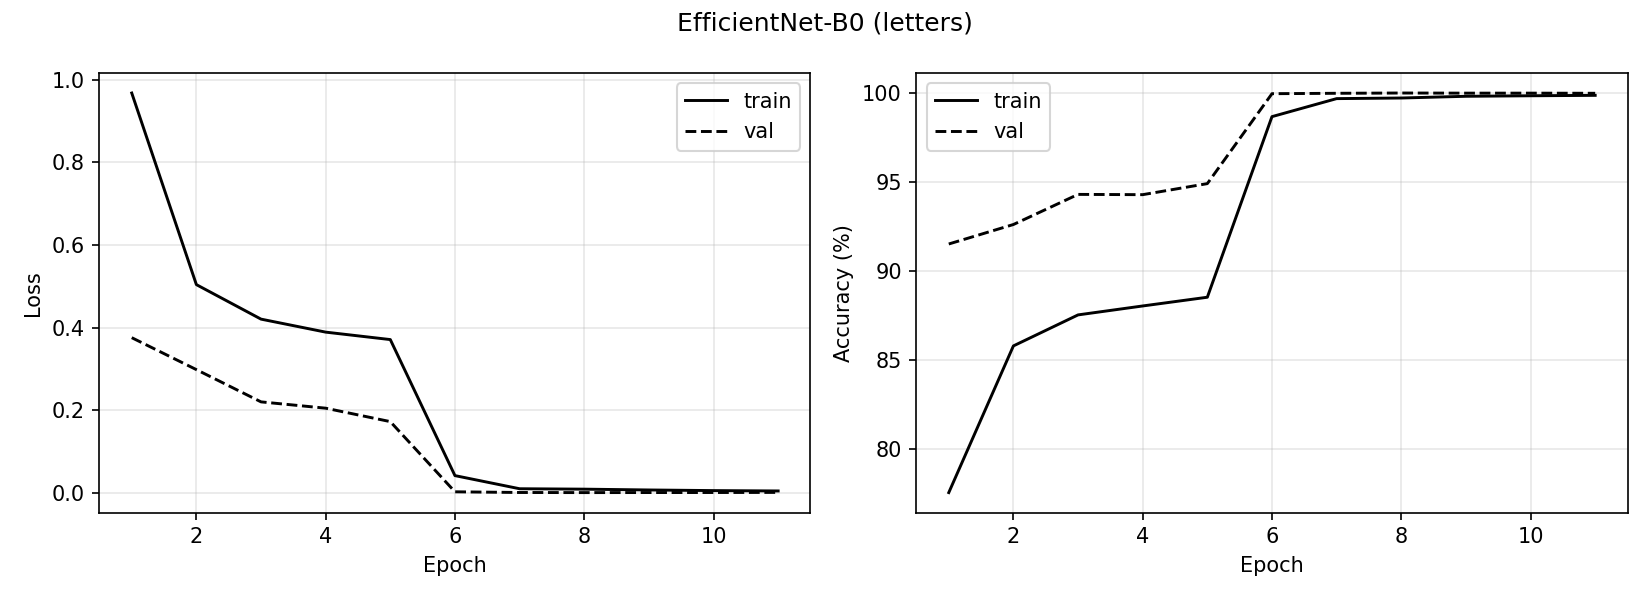
\includegraphics[width=\textwidth]{figures/ch5_lc_cnn.png}
\caption{Training trajectory of the EfficientNet-B0 letter
classifier. Both train and validation loss collapse within the
first six epochs and validation accuracy saturates at
\SI{100}{\percent} from epoch~7 onward, which triggered the
early-stopping criterion at epoch~11. The narrow train--val gap
indicates that no overfitting developed despite the large
\num{60900}-image training partition.}
\label{fig:results-lc-cnn}
\end{figure}

\begin{figure}[h]
\centering
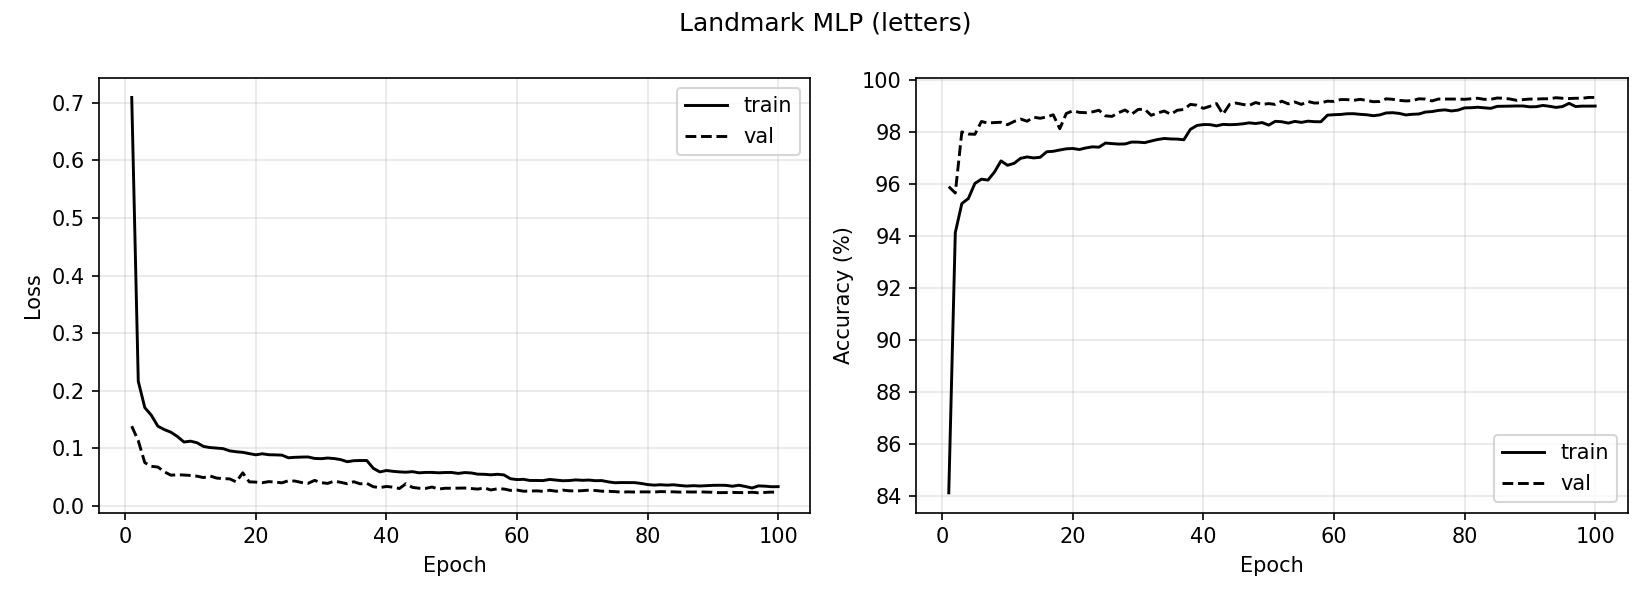
\includegraphics[width=\textwidth]{figures/ch5_lc_mlp.png}
\caption{Training trajectory of the landmark MLP letter
classifier. Validation accuracy crosses \SI{98}{\percent} within
the first ten epochs and plateaus near \SI{99.3}{\percent} for the
remaining \num{90} epochs. The validation curve remains
consistently above the training curve throughout, which is the
expected pattern when dropout regularisation is active during
training but disabled at inference.}
\label{fig:results-lc-mlp}
\end{figure}

\begin{figure}[h]
\centering
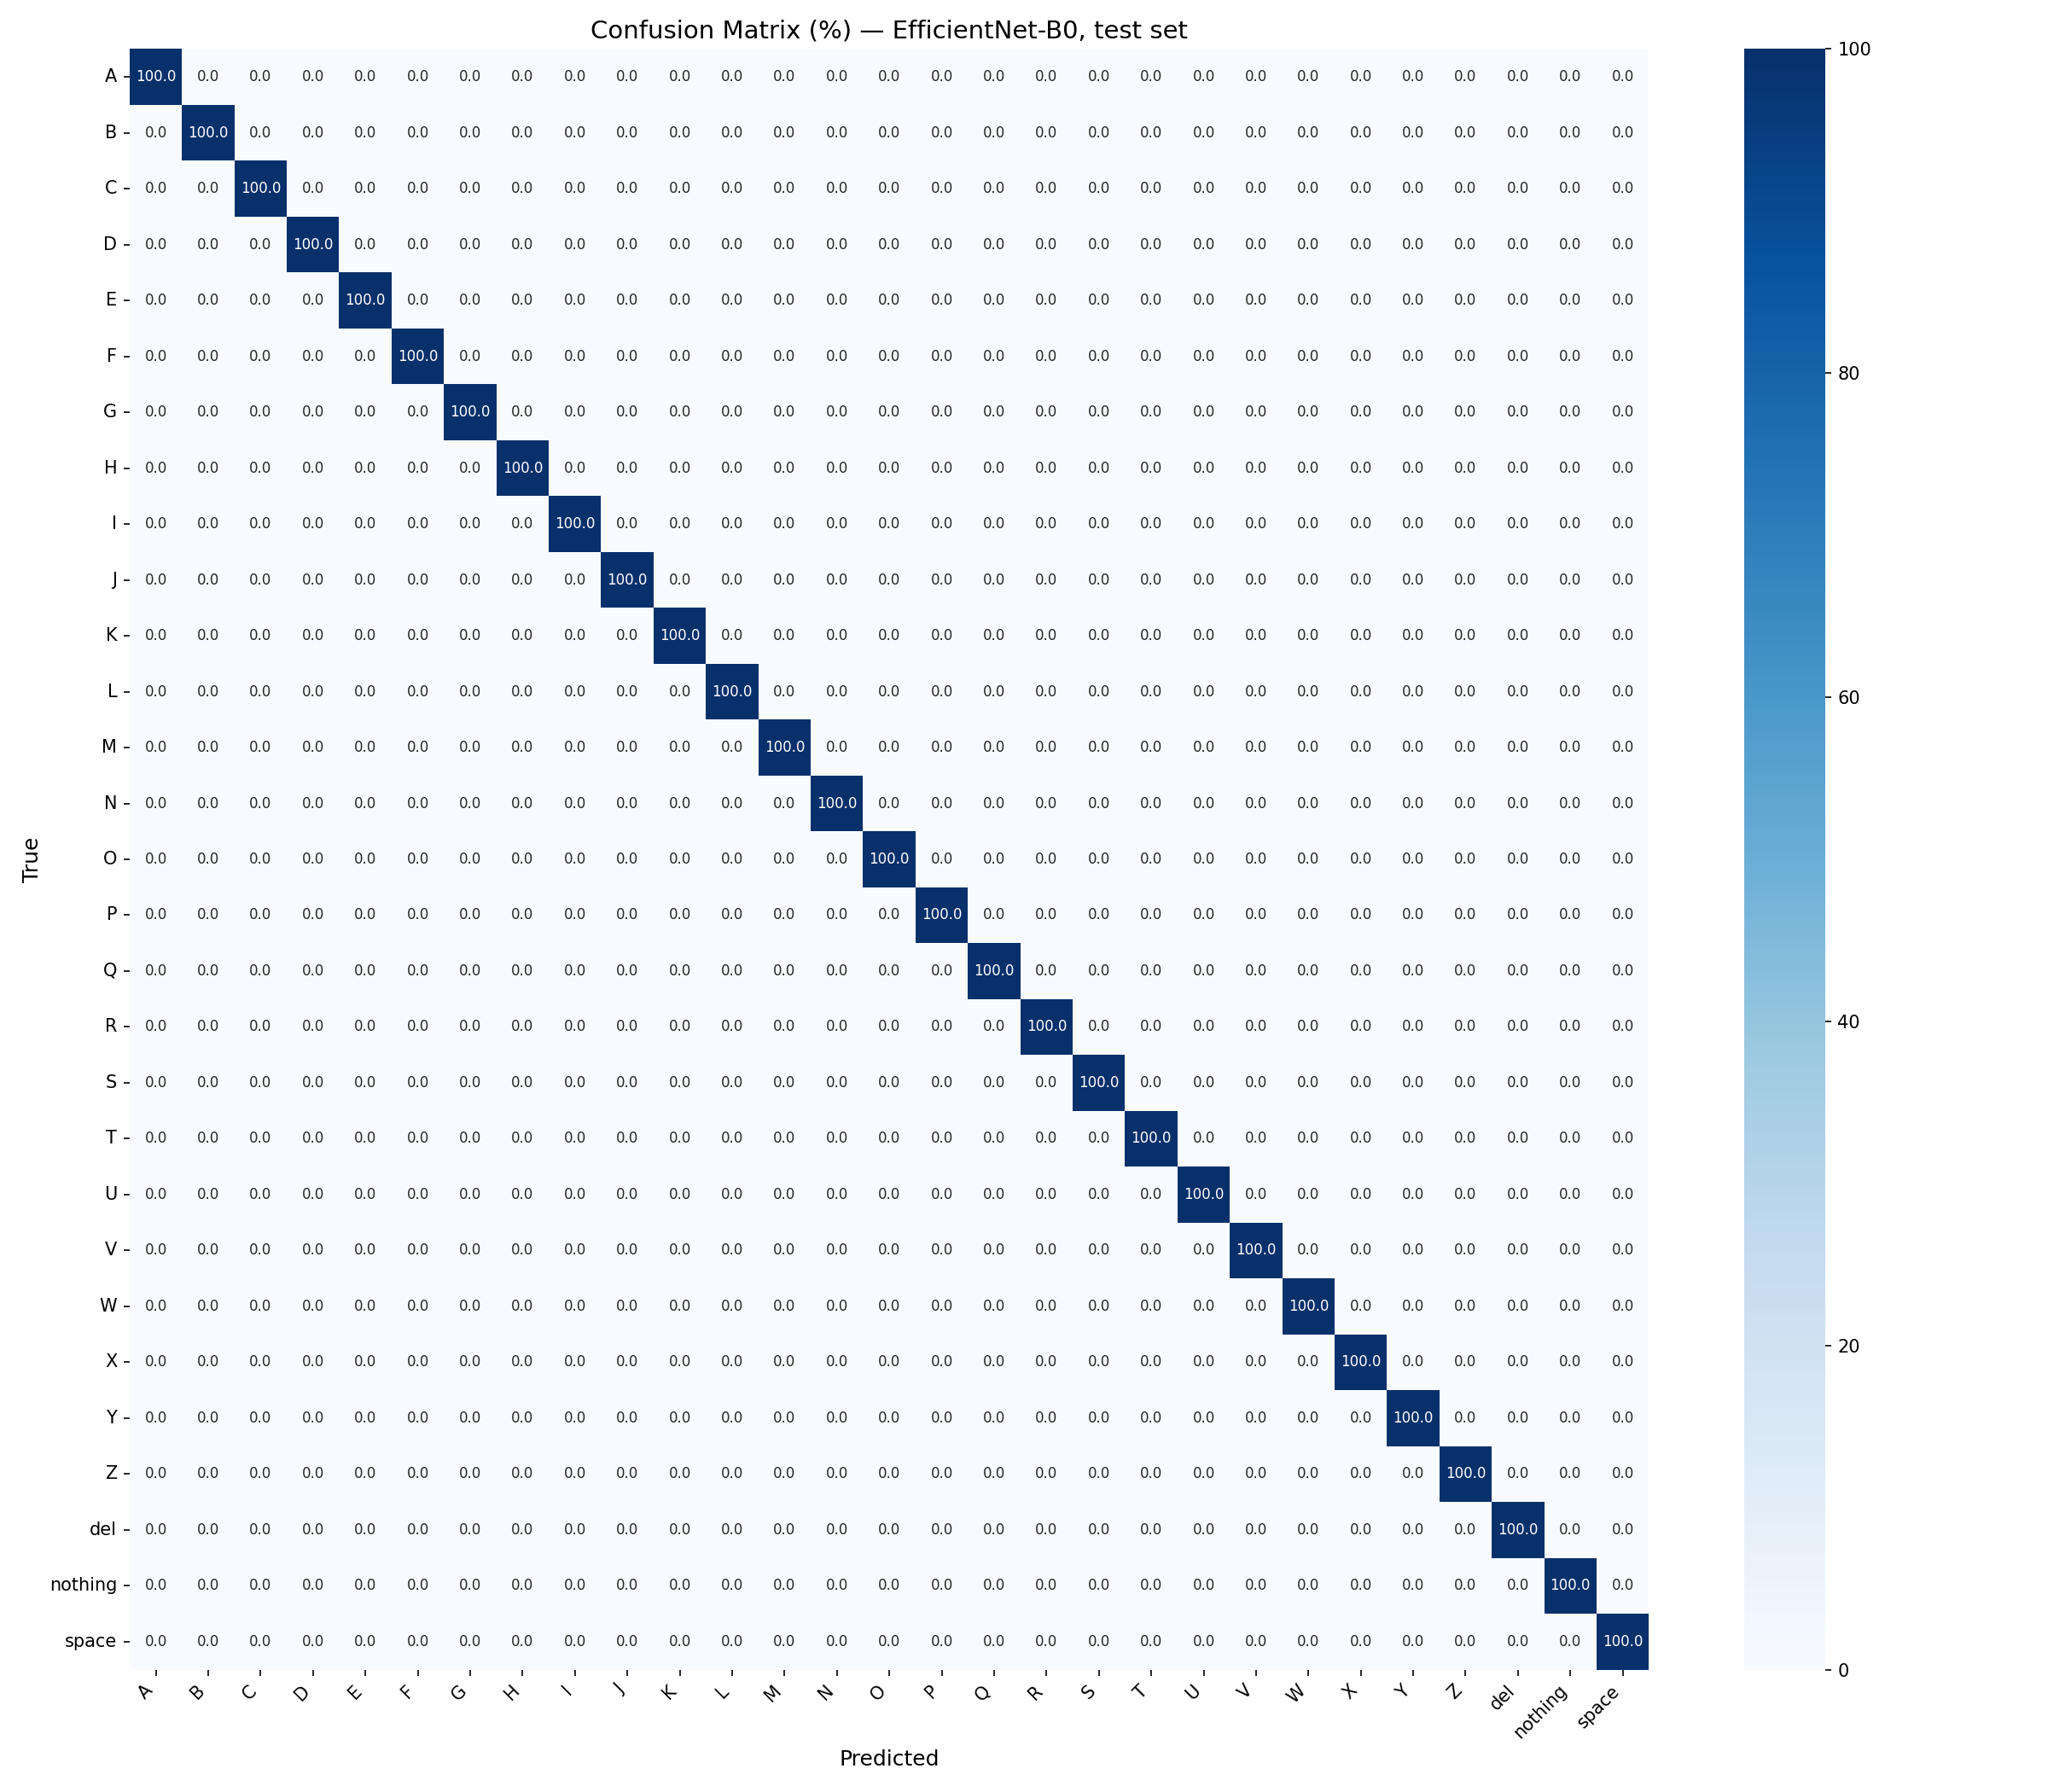
\includegraphics[width=0.9\textwidth]{figures/ch5_cm_cnn_letters.png}
\caption{Row-normalised confusion matrix of the EfficientNet-B0
letter classifier on the 13\,050-image ASL Alphabet test partition.
Cells report the percentage of true class~$y$ predicted as
class~$\hat{y}$. The matrix is strictly diagonal: the network
produces zero off-diagonal predictions across all 29 classes,
matching the 100\,\% Top-1 accuracy of
Table~\ref{tab:results-letters}.}
\label{fig:results-cm-cnn}
\end{figure}

\begin{figure}[h]
\centering
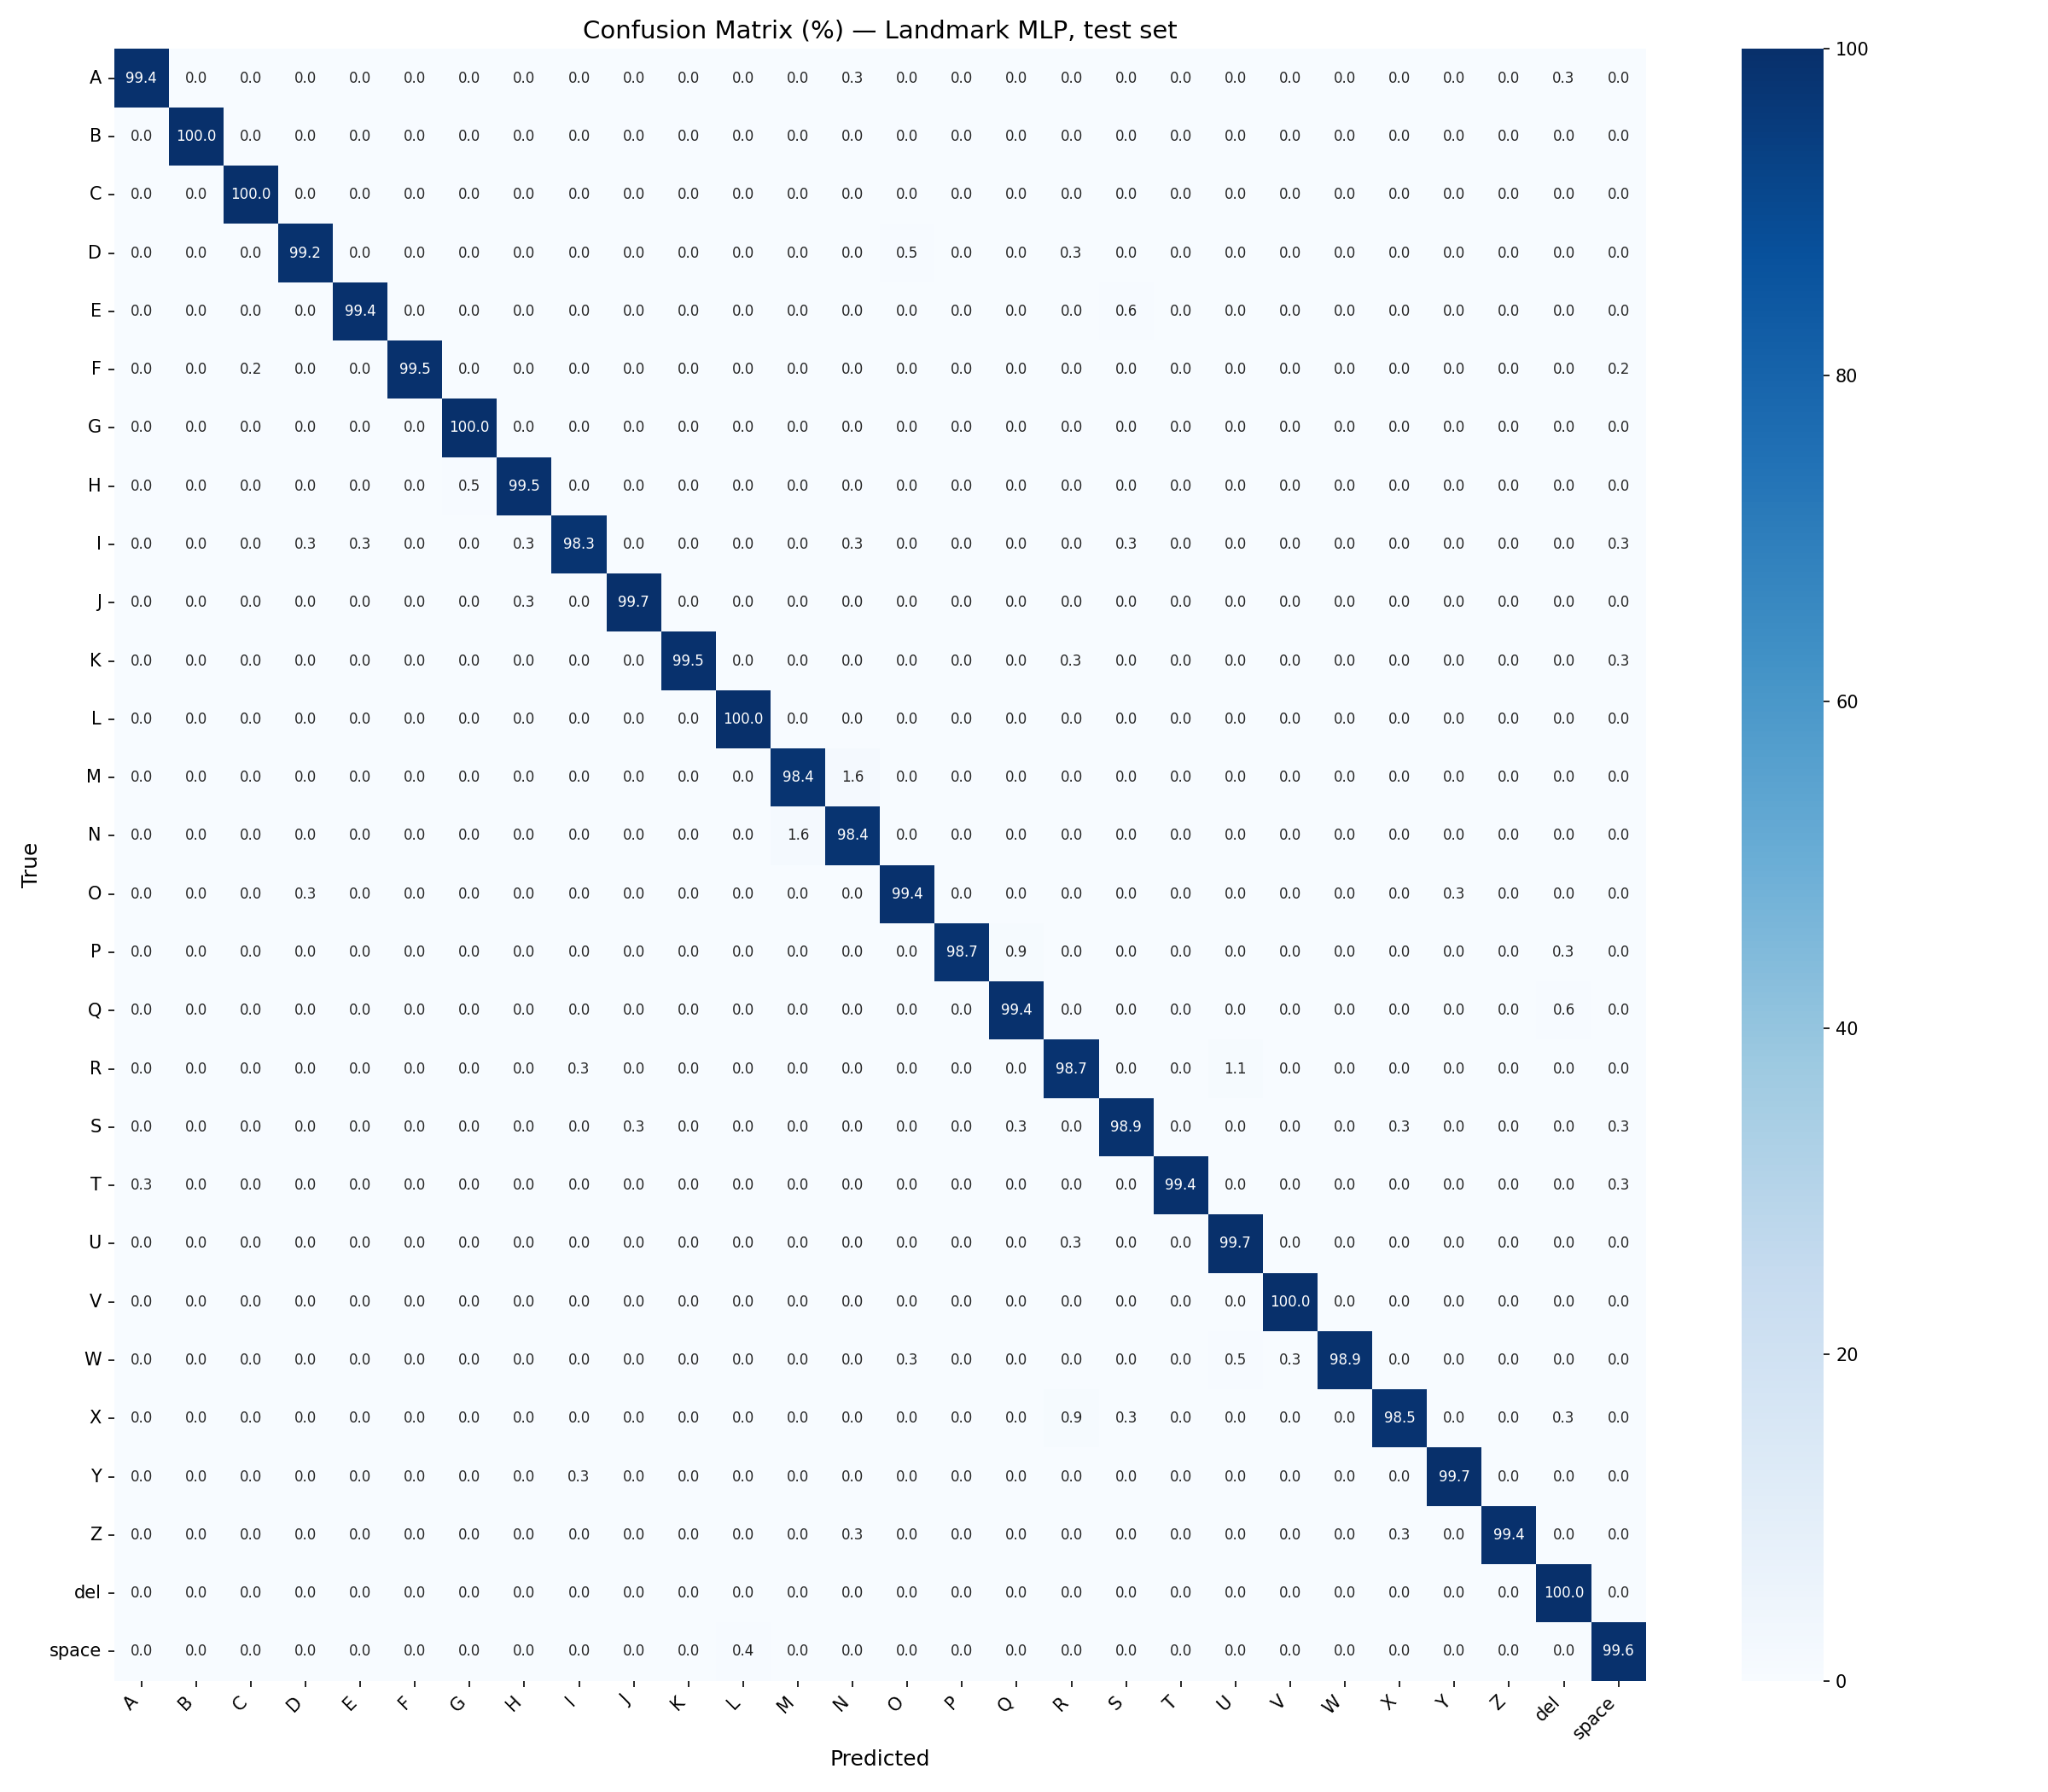
\includegraphics[width=0.9\textwidth]{figures/ch5_cm_mlp_letters.png}
\caption{Row-normalised confusion matrix of the landmark MLP letter
classifier on the detector-recoverable subset of the ASL Alphabet
test partition (73.09\,\% coverage). The matrix is dominated by the
diagonal; off-diagonal cells remain below \SI{2}{\percent} and
concentrate around classes whose handshape MediaPipe captures less
reliably, in particular the thumb-tucked \textit{M}/\textit{N} pair
and the closely related \textit{R}/\textit{U}/\textit{V} group.}
\label{fig:results-cm-mlp}
\end{figure}

Two observations carry over to Chapter~\ref{ch:conclusion}. The first
is that on this dataset the image network is the more reliable choice
because it runs on every input image, whereas the landmark network is
effectively gated on MediaPipe's detection. The 26.91\,\% of test
images on which MediaPipe failed include the entire \texttt{nothing}
class (which contains no hand by construction) and a subset of the
letters~\textit{M} and~\textit{N}, whose thumb-tucked hand-shape
defeats the detector on low-resolution crops. The on-device demo
preserves this asymmetry: the image classifier always produces an
output, while the landmark classifier displays a faded ``no hand
visible'' marker on frames where MediaPipe finds no hand.

The second observation is that the two classifiers occupy opposite
ends of the size/speed trade-off explored in this thesis. The MLP is
65$\times$ smaller and roughly two orders of magnitude faster than
EfficientNet at offline throughput, while losing 0.62 percentage
points of accuracy on the images where it is defined. For practical
mobile deployment, the relevant question is not which of these two
absolute numbers is larger but which configuration is appropriate
under a given resource budget; the on-device measurements of
Section~\ref{sec:results-on-device} answer that question
quantitatively.

A third observation tempers both of the previous ones: the perfect
test accuracy of the image network and the near-perfect accuracy of
the landmark network are not predictions of real-world performance.
Both numbers were obtained on a random split of a single-source
dataset whose images were collected in a controlled setting by a
single contributor on Kaggle. Section~\ref{sec:results-on-device}
reports the substantially noisier behavior of both classifiers when
they are pointed at a new hand under the natural lighting and
background variation of a smartphone camera; the gap between offline
test accuracy and on-device accuracy is the appropriate measure of
how well each model would generalize in production use.

%==============================================================================
\section{Word Recognition Results}
\label{sec:results-words}

The word classifier is evaluated against the five-seed protocol described
in Section~\ref{sec:results-methodology}: five independently trained
BiLSTM instances and a five-seed ensemble that averages their pre-softmax
logits. All six checkpoints are evaluated once on the held-out 201-clip
WLASL-100 test partition. Per-seed scores establish the variance baseline
of the single-model variant; the ensemble line in
Table~\ref{tab:results-words-seeds} is the model that the Android demo
exposes as ``BiLSTM Ensemble (x5)''.

\begin{table}[h]
\centering
\caption{Per-seed and ensemble accuracy on the WLASL-100 test set.}
\label{tab:results-words-seeds}
\begin{tabular}{lccc}
\toprule
\textbf{Model} & \textbf{Top-1 (\%)} & \textbf{Top-5 (\%)} & \textbf{Macro F1} \\
\midrule
BiLSTM seed 0           & 53.23 & 80.60 & 0.491 \\
BiLSTM seed 1           & 52.74 & 78.11 & 0.495 \\
BiLSTM seed 2           & 56.22 & 79.10 & 0.524 \\
BiLSTM seed 3           & 49.75 & 77.61 & 0.447 \\
BiLSTM seed 4           & 48.76 & 79.60 & 0.469 \\
\midrule
Five-seed mean          & 52.14 & 79.00 & 0.485 \\
Five-seed range         & $\pm$3.73 & $\pm$1.49 & $\pm$0.038 \\
\midrule
\textbf{Ensemble (logit avg.)} & \textbf{56.22} & \textbf{81.09} & \textbf{0.521} \\
\bottomrule
\end{tabular}
\end{table}

The training trajectory underlying these numbers is reported in
Figure~\ref{fig:results-lc-lstm}. All five seeds follow the same
overall shape: a steep loss drop and accuracy climb during the
first roughly forty epochs, followed by a long tail of slow
improvement. Seed-to-seed variance is visible throughout but
narrows in the second half of training as the curves converge
toward the band centred on the five-seed mean. Two of the five
seeds triggered the early-stopping criterion before epoch~100,
which is why the per-seed lines terminate at different epochs.
The smoother bold curve is the mean across the overlapping epoch
range and corresponds to the average single-seed trajectory whose
endpoint matches the per-seed mean of
Table~\ref{tab:results-words-seeds}.

\begin{figure}[h]
\centering
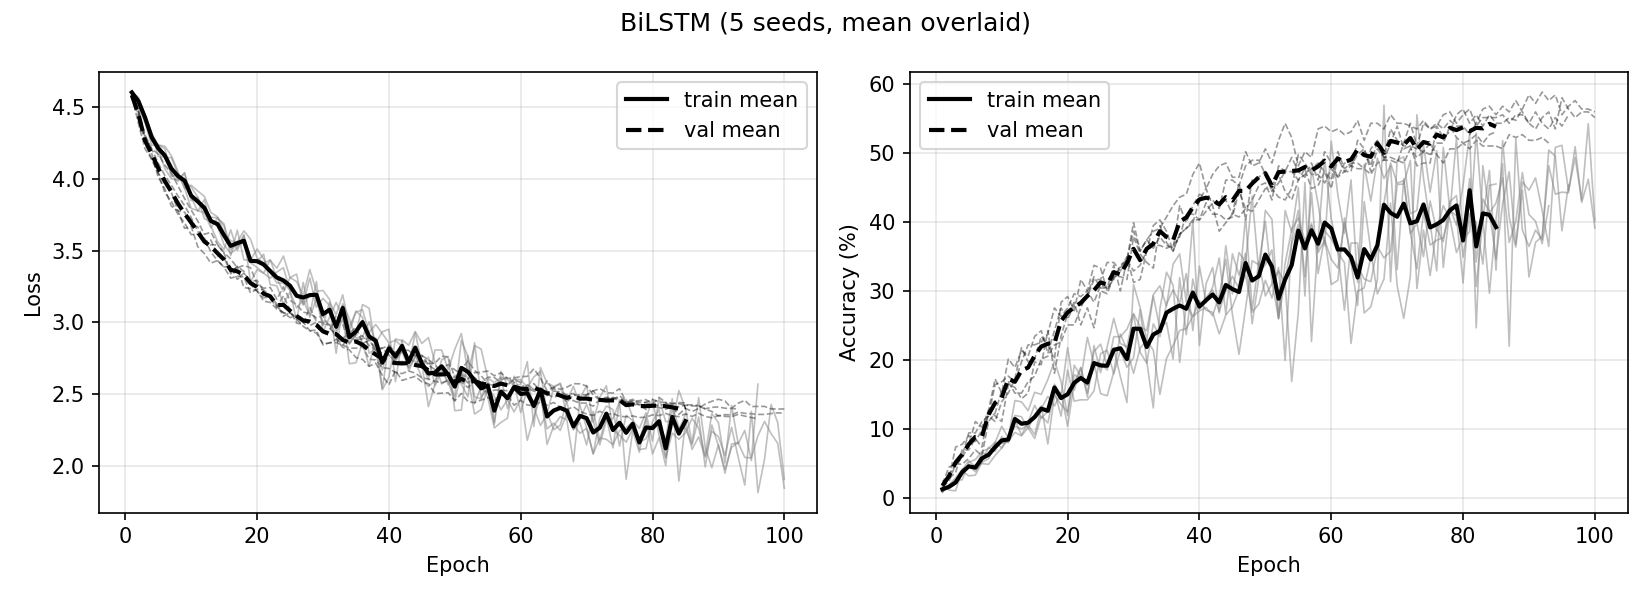
\includegraphics[width=\textwidth]{figures/ch5_lc_lstm.png}
\caption{Training trajectories of the five BiLSTM seeds trained
under the V2 configuration. Thin grey lines are individual seeds,
the bold black lines are the per-epoch mean across seeds (averaged
over the epoch range on which all seeds were still active).}
\label{fig:results-lc-lstm}
\end{figure}

The single-seed Top-1 accuracy varies by roughly four percentage points
across the five runs, which is consistent with the limited test
partition size of 201 clips: a single misclassification moves Top-1 by
0.50 points, so seed-level variance of $\pm 3$--$4$ points is expected
rather than alarming. The ensemble lifts Top-1 from 52.14\,\% (the
five-seed mean) to 56.22\,\% and Top-5 from 79.00\,\% to 81.09\,\%, in
line with the textbook expectation that averaging decorrelated
predictors increases accuracy at the cost of a proportional increase in
inference compute~\cite{dietterich2000ensemble}. Equally important, the
ensemble matches the best single seed exactly on Top-1: the seed~2 run
also reaches 56.22\,\%, but on a different subset of the test clips
than the ensemble, so the two methods do not produce identical predictions.

\subsection{Comparison with Proposal Acceptance Criteria}
\label{sec:results-words-acceptance}

The project proposal defines two thresholds for the word task: a hard
acceptance criterion of Top-1 $\geq 40\,\%$ and a stretch target of
Top-1 $\geq 60\,\%$ on the same test partition. The ensemble result of
56.22\,\% clears the acceptance criterion by 16.22 percentage points
and reaches within 3.78 percentage points of the stretch target. The
gap to the stretch target is consistent with the validation accuracy
of 60.08\,\% reported in Section~\ref{sec:impl-lstm-ensemble}: the
ensemble crosses 60\,\% on the validation set but loses approximately
four points on the smaller and more variable test set, which is the
common pattern observed across deep-learning evaluations on
limited-size data.

\subsection{Position in the WLASL-100 Literature}
\label{sec:results-words-literature}

Table~\ref{tab:results-wlasl-lit} places the ensemble's 56.22\,\% Top-1
against published results on the same WLASL-100 split. The comparison
is necessarily approximate because reported numbers use different
input modalities, preprocessing pipelines and hardware budgets;
nevertheless, the table communicates the relative position of a
hands-only landmark model among the available approaches.

\begin{table}[h]
\centering
\caption{Reported Top-1 accuracy on the WLASL-100 test split. Numbers
are quoted from each publication; the modality column distinguishes
RGB, body pose, body+hand pose and hand-only inputs.}
\label{tab:results-wlasl-lit}
\begin{tabular}{llll}
\toprule
\textbf{Year} & \textbf{Method} & \textbf{Modality} & \textbf{Top-1 (\%)} \\
\midrule
2020 & I3D~\cite{li2020wlasl}              & RGB                & 65.89 \\
2020 & Pose-TGCN~\cite{li2020wlasl}        & Body pose          & 55.43 \\
2020 & VGG-GRU~\cite{li2020wlasl}          & RGB                & 25.97 \\
2020 & TK-3D ConvNet~\cite{li2020transferring} & RGB (+ web news transfer) & 77.55 \\
2021 & Fusion-3~\cite{hosain2021fusion}    & RGB + body pose    & 75.67 \\
2022 & SPOTER~\cite{bohacek2022spoter}     & Body+hand pose     & 63.18 \\
\midrule
\textbf{2026} & \textbf{This work (BiLSTM ensemble)} & \textbf{Hands only} & \textbf{56.22} \\
\bottomrule
\end{tabular}
\end{table}

Two observations frame the result. First, the RGB-based pipelines
operate on a substantially heavier input pipeline---raw video
frames---and produce model sizes that are an order of magnitude
larger than 5.51\,MB. The hands-only configuration sacrifices roughly
10 points of Top-1 accuracy relative to the single-stream I3D baseline,
and just over 20 points against the strongest reported method on
WLASL-100---the cross-domain TK-3D ConvNet of Li et al., which
augments I3D with knowledge transferred from subtitled news
videos---in exchange for a 200~ms inference budget on a phone CPU.
Second, when the comparison is restricted to landmark-only methods,
the result is competitive: the ensemble is within one point of the
body-pose Pose-TGCN baseline and within seven points of the
transformer-based SPOTER, despite using a smaller architecture and a
strictly smaller input feature set (21 hand landmarks per frame,
against 55 upper-body keypoints for Pose-TGCN and 54 head-body-hand
landmarks for SPOTER). The trade-off
characterized in Chapter~\ref{ch:implementation} therefore plays out
as expected on the offline benchmark: heavier RGB or multi-stream
pipelines win on accuracy, lighter landmark pipelines win on
deployability, and the present model occupies an intentional point
on that curve.

\subsection{Inference Latency}
\label{sec:results-words-latency}

Offline inference latency for the BiLSTM single model is
1.87\,ms per sample on the training GPU, corresponding to a throughput
of 534 frames per second on the same hardware. The ensemble inflates
this by approximately a factor of five, in line with the
five-checkpoint structure; on the same GPU the ensemble reaches roughly
110~FPS at an end-to-end latency of 9~ms. Both numbers are well above
the proposal's non-functional requirement of 10~FPS
(NFR-04) on the offline machine. The corresponding on-device numbers,
which include the MediaPipe landmark stage and run on the Android test
phone, are reported in Section~\ref{sec:results-on-device}; they are
the deployment-relevant numbers.

%==============================================================================
\section{Ablation Study}
\label{sec:results-ablation}

The word classifier reported in Section~\ref{sec:results-words} did not
arrive at 56.22\,\% Top-1 in a single step. An earlier configuration
(referred to internally as~V1) was trained with single-hand input,
without sequence-level augmentation and without ensemble averaging; it
reached only 20.00\,\% validation accuracy on the same WLASL-100 split.
The remaining 36 percentage points were gained incrementally over six
modifications which together define the V2 configuration described in
Section~\ref{sec:impl-lstm}. Table~\ref{tab:results-ablation} summarizes
the trajectory and is the single most useful artefact for understanding
which design choices carried the most weight on this dataset.

\begin{table}[h]
\centering
\caption{Incremental ablation from the V1 baseline to the V2 ensemble.
Validation accuracy is reported because the test set was kept frozen
until the final V2 configuration had been selected; the bottom row
reports the corresponding test accuracy that
Section~\ref{sec:results-words} discusses in detail.}
\label{tab:results-ablation}
\begin{tabular}{clcc}
\toprule
\textbf{Step} & \textbf{Added component} & \textbf{Val Top-1 (\%)} & \textbf{$\Delta$} \\
\midrule
0 & V1 baseline (single hand, no augmentation)        & 20.00 & --- \\
1 & + WLASL \texttt{frame\_start}/\texttt{frame\_end} crop & (bundled) & (bundled) \\
2 & + two-hand extraction with presence flags         & (bundled) & (bundled) \\
3 & + sequence augmentation\textsuperscript{a}        & 47.33     & +27.33 \\
4 & + mixup ($\alpha=0.2$)                            & (bundled) & (bundled) \\
5 & + hidden size 128 $\rightarrow$ 192               & (bundled) & (bundled) \\
6 & + time-scaling $\pm 20\,\%$                       & (bundled) & (bundled) \\
7 & + \texttt{WeightedRandomSampler}                  & 54.32 & +6.99 \\
8 & + mixup $\alpha$ 0.2 $\rightarrow$ 0.4            & 58.85 & +4.53 \\
9 & + five-seed ensemble (logit averaging)            & \textbf{60.08} & +1.23 \\
\midrule
\multicolumn{2}{l}{\textbf{Test set (V2 ensemble)}}    & \multicolumn{2}{c}{\textbf{56.22 / 81.09 (Top-1 / Top-5)}} \\
\bottomrule
\end{tabular}
\\[0.4em]
\footnotesize\textsuperscript{a}Temporal jitter $\pm 4$ frames, frame dropout $p{=}0.15$, Gaussian noise $\sigma{=}0.02$.
\end{table}

Steps~1--6 were applied as a single ``data and architecture'' bundle
during V2 development, so the table reports the marginal effect of the
bundle (step~3, +27.33 points) rather than that of each individual
component. The decision to bundle these modifications was deliberate:
each one targets a different failure mode of V1 (frame-window noise,
missing second hand, identical input sequences across epochs,
underparameterized recurrent state, fixed-length sampling) and
isolating them would have multiplied the training budget for a
question that the proposal does not require us to answer. A finer
component-level ablation is listed as future work in
Chapter~\ref{ch:conclusion}.

The remaining three rows isolate single decisions and warrant separate
comment. The \texttt{WeightedRandomSampler} (step~7, +6.99 points)
re-balances the loss against the long tail of WLASL-100, where the
majority of words have between one and four training clips; without
this sampler the model collapses onto the head classes and the macro
F1 score drops noticeably even when Top-1 stays competitive. Increasing
the mixup intensity from $\alpha = 0.2$ to $\alpha = 0.4$ (step~8,
+4.53 points) increases the regularization pressure and is what closed
most of the remaining single-seed gap to the proposal stretch target;
the choice was guided by the validation curves, which showed the
$\alpha = 0.2$ run beginning to overfit around epoch 60. The five-seed
ensemble (step~9, +1.23 points on the validation set and +4.08 points
relative to the five-seed mean of 52.14\,\% on the test set, as
discussed in Section~\ref{sec:results-words}) is the cheapest source of
accuracy in the entire pipeline---the additional cost is purely at
inference time and is bounded by the five-fold latency penalty
quantified in Section~\ref{sec:results-on-device}.

%==============================================================================
\section{Error Analysis}
\label{sec:results-errors}

A model that reaches 56.22\,\% Top-1 also misclassifies 43.78\,\% of
the WLASL-100 test clips. Whether those errors are random or
structured is the more interesting question and is what this section
addresses. Figure~\ref{fig:results-cm-words} visualises the
ensemble's row-normalised confusion matrix on the 25 most populous
classes of the WLASL-100 test partition; the remaining 75 classes
each contribute at most a single test clip and are omitted to keep
the matrix legible. The matrix is dominated by a clear diagonal,
with the two visible off-diagonal cells (\texttt{woman}\,$\to$\texttt{fine},
\texttt{last}\,$\to$\texttt{before}) corresponding to signs that
share location or motion with their misclassified target. The
matrix of the ensemble was inspected systematically for the
five most frequent confusion pairs across the full 100-class
matrix; the result is summarised in
Table~\ref{tab:results-confusions}. None of the five pairs are random.
Each one corresponds to a pair of ASL signs that share a handshape, a
location on the body or a movement trajectory, and the model's mistakes
therefore look like the mistakes a beginning ASL student would make
rather than like the noise of an under-trained network.

\begin{table}[h]
\centering
\caption{Five most frequent confusion pairs in the ensemble predictions,
with the linguistic reason for the visual ambiguity.}
\label{tab:results-confusions}
\begin{tabular}{llp{7.4cm}}
\toprule
\textbf{Ground truth} & \textbf{Prediction} & \textbf{Reason for visual similarity} \\
\midrule
\texttt{black}  & \texttt{who}   & Both one-handed; index-finger motion near the head and cheek. \\
\texttt{dog}    & \texttt{later} & Both one-handed; finger-snap motion with the same handshape transition. \\
\texttt{change} & \texttt{how}   & Both two-handed; rotating-fist handshape with bilateral movement. \\
\texttt{want}   & \texttt{many}  & Both two-handed; fingers open from a closed configuration. \\
\texttt{mother} & \texttt{fine}  & 5-handshape with thumb contact on chin or forehead in both signs. \\
\bottomrule
\end{tabular}
\end{table}

\begin{figure}[h]
\centering
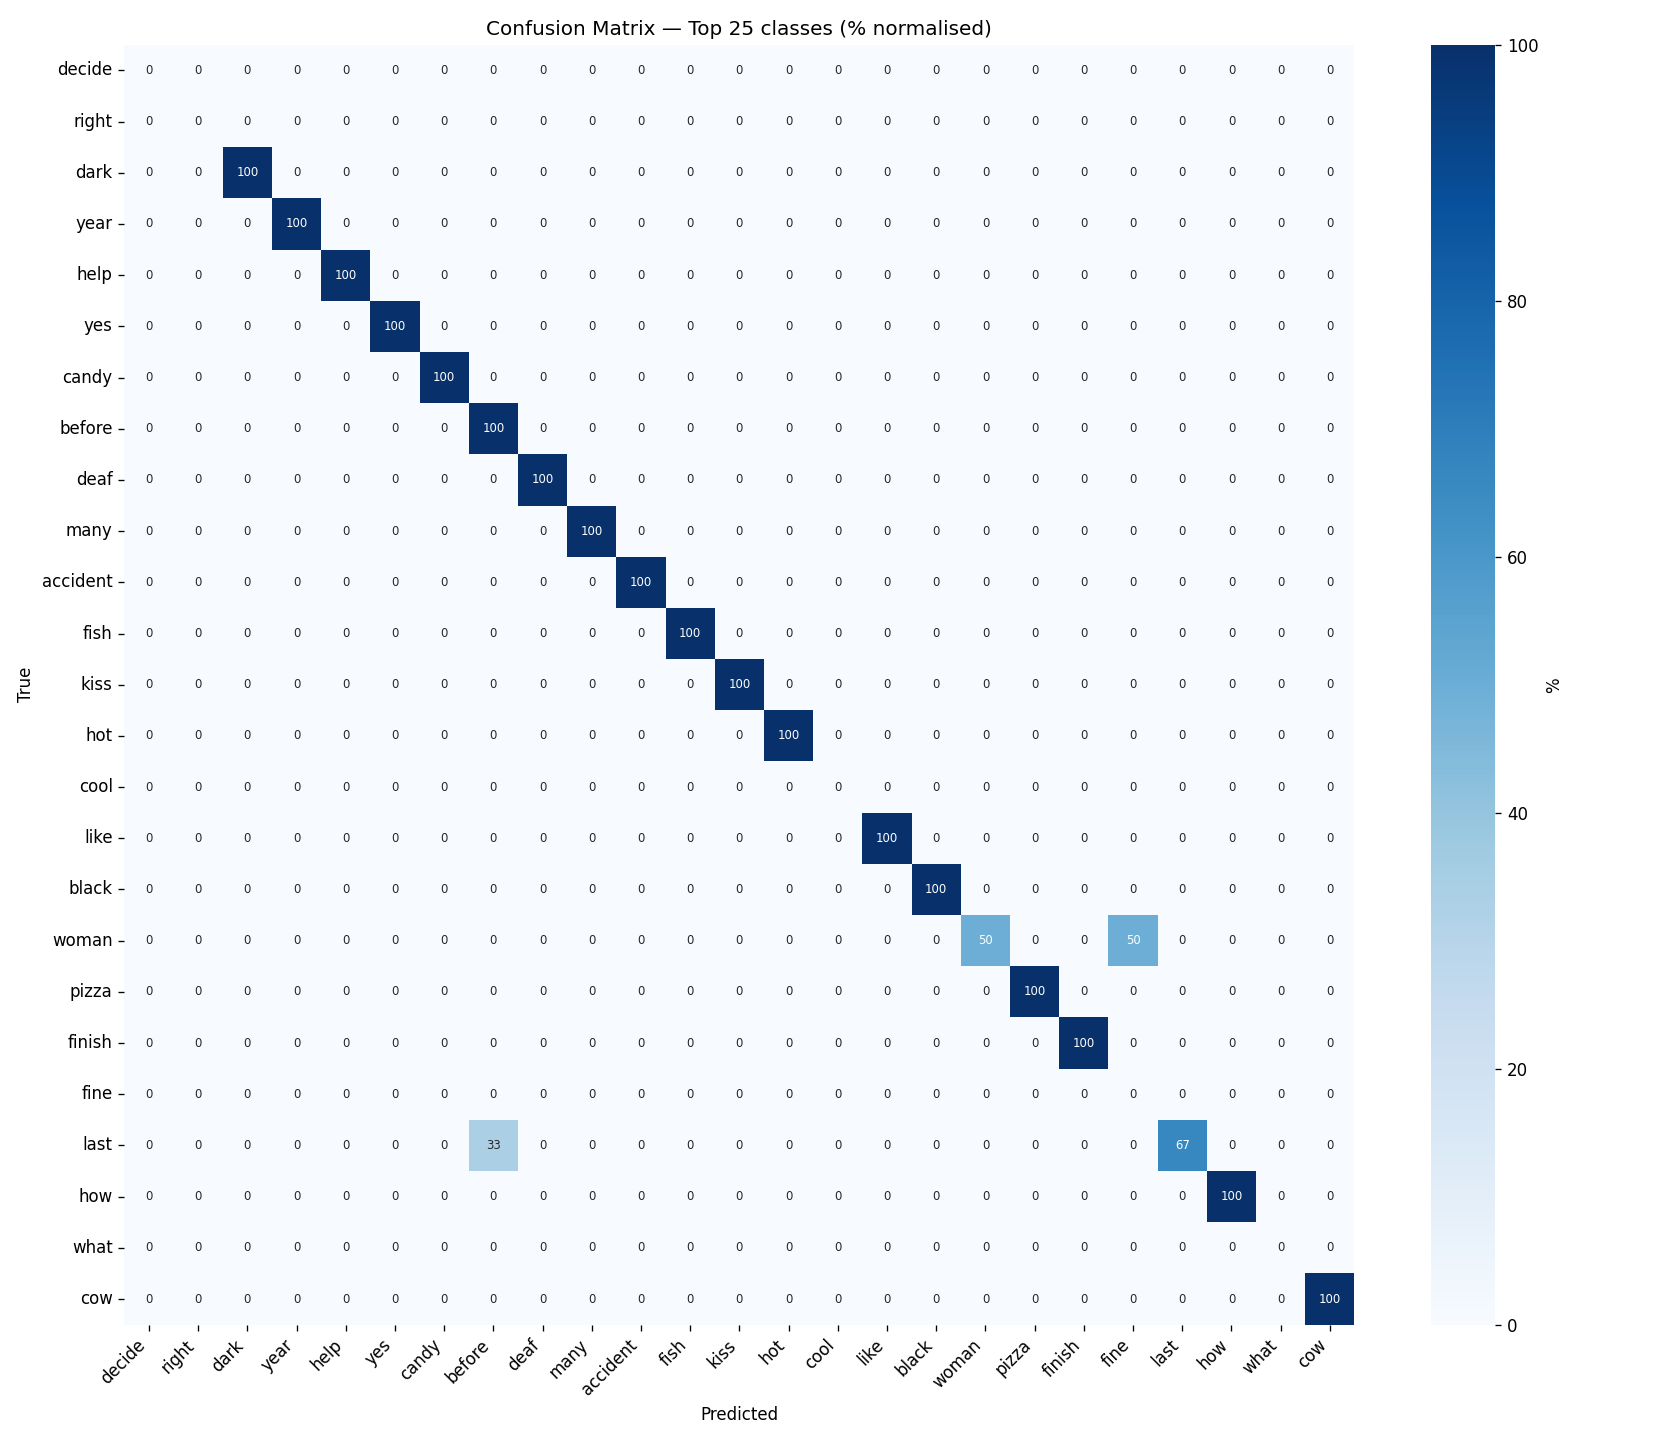
\includegraphics[width=\textwidth]{figures/ch5_cm_lstm_words.png}
\caption{Row-normalised confusion matrix of the five-seed BiLSTM
ensemble on the 25 most populous classes of the WLASL-100 test
partition. The full 100-class matrix is dominated by single-clip
rows that are not visually informative; the truncation to the top
25 classes by test support preserves the diagonal-with-isolated-confusions
structure of the prediction error.}
\label{fig:results-cm-words}
\end{figure}

The implication of the table is that the model has internalized the
high-level structure of an ASL sign (handedness, location and the
class of movement) and fails on the fine-grained handshape or
trajectory details that distinguish minimally different signs. From a
sign-language-linguistic perspective this is the expected failure
mode of a hands-only model: pose information about the arm and torso
would resolve several of these confusions, and facial markers would
resolve others (the distinction between \texttt{mother} and
\texttt{fine}, in particular, is partly tied to a facial component
that hand landmarks cannot capture). The Limitations subsection of
Chapter~\ref{ch:conclusion} returns to this point in the context of
multi-stream models that combine hand, body and facial input.

Two structural caveats round out the error picture. First, two of the
hundred WLASL-100 classes (\texttt{later} and \texttt{book}) have
\emph{zero} examples in the official test partition because the
canonical split allocates their few available clips to train and
validation. The macro F1 score of 0.521 reported in
Table~\ref{tab:results-words-seeds} therefore averages over the
98~effective classes that have at least one test clip, rather than
over the full 100. This is a property of the WLASL-100 evaluation
protocol, not of the model. Second, the Top-5 accuracy of 81.09\,\%
combined with a Top-1 accuracy of 56.22\,\% means that the correct
label is among the top five predictions in roughly 25 percentage
points of clips that the Top-1 metric counts as failures. In a
real-world interactive application this gap is recoverable through a
``did you mean'' interaction surface (a confidence-ranked shortlist of
candidate signs); the Android demo of Chapter~\ref{ch:implementation}
does not implement such a surface but the option is preserved for
future work.

%==============================================================================
\section{On-Device Performance}
\label{sec:results-on-device}

The offline numbers reported in
Sections~\ref{sec:results-letters}--\ref{sec:results-words} are measured
on the training GPU and are useful for cross-checking the model against
the published literature, but they do not characterise the system that
the proposal actually promised to deliver: an Android application that
runs the classifiers on-device, displays the recognised letter or word
and reports its own throughput and latency. This section reports the
on-device counterparts of those numbers, measured directly on two
mid-tier Android phones during the manual test described in
Section~\ref{sec:results-qualitative}.

\subsection{Test Devices and Protocol}
\label{sec:results-on-device-protocol}

Two phones were used in the manual test. The first, a
\textbf{TECNO~SPARK 20C}, is an entry-level device built around a
MediaTek Helio~G36 SoC (8\,nm, 8 ARM Cortex-A53 cores at up to
\SI{2.2}{\giga\hertz}, 8\,GB RAM, Android~13). It represents the
budget segment of the Android market on which an accessibility tool
must remain usable. The second, a \textbf{Xiaomi~15T~Pro}, is a
2025-generation flagship built around a MediaTek Dimensity~9400+ SoC
(3\,nm, 1+3+4 cluster topology with an ARM Cortex-X925 prime core,
12\,GB LPDDR5X RAM, Android~15) and represents the upper end of the
deployable hardware. Both devices ran the same APK
(\texttt{./gradlew installDebug}, commit \texttt{b1d5465} plus the
Words single-shot lock changes of Section~\ref{sec:impl-android-pipeline})
under matched conditions: daylight illumination from a window, a
neutral background, and a hand-to-camera distance of
\SIrange{30}{50}{\centi\metre}. Battery Saver was disabled on both
devices to prevent CPU throttling from contaminating the measurement.

For each of the four classifiers, the relevant tab of the application
was opened, a static target (a single letter for the letter models, a
single fixed word for the word models) was held in front of the camera
for \SI{60}{\second}, and the on-screen FPS and latency badges were
read every ten seconds from a screen recording, producing six samples
per model and device. The badge reports the end-to-end pipeline
latency measured inside the analyzer: camera frame
$\rightarrow$ MediaPipe Hands $\rightarrow$ classifier
$\rightarrow$ UI publication. It is therefore the deployment-relevant
quantity, not an isolated model-inference number. To avoid a
device-mismatch confound the letter models were measured on both
phones; the word models were measured on both phones initially, but
on the TECNO the ensemble produced latencies that made the application
unusable (Section~\ref{sec:results-on-device-words}), so the Words
qualitative test of Section~\ref{sec:results-qualitative} was carried
out exclusively on the Xiaomi.

\subsection{Letter Models}
\label{sec:results-on-device-letters}

Table~\ref{tab:on-device-letters} reports the six-sample mean,
minimum and maximum FPS and latency for the two letter classifiers on
both devices. Two patterns emerge clearly. On the Xiaomi 15T~Pro both
classifiers saturate the camera at \SI{30}{FPS} with latencies well
inside the proposal's non-functional budget (NFR-04, \SI{10}{FPS}
end-to-end on the offline machine). On the TECNO SPARK~20C only the
landmark MLP keeps the pipeline within a real-time budget; the
image-based EfficientNet stays at a respectable \SI{20.7}{FPS}
average, but the end-to-end latency rises to \SI{203}{ms} mean and
peaks at \SI{220}{ms}, an order of magnitude higher than its Xiaomi
counterpart.

\begin{table}[h]
\centering
\caption{On-device throughput and latency of the two letter
classifiers, measured from the in-app FPS/latency badge over a
60-second window (six samples per cell).}
\label{tab:on-device-letters}
\resizebox{\textwidth}{!}{%
\begin{tabular}{llccccc}
\toprule
\textbf{Model} & \textbf{Device} & \textbf{Mean FPS} & \textbf{Min FPS} & \textbf{Max FPS} & \textbf{Mean lat.\ (ms)} & \textbf{Max lat.\ (ms)} \\
\midrule
EfficientNet-B0 & Xiaomi 15T Pro   & 30.0 & 30 & 30 & 35.2 & 40 \\
EfficientNet-B0 & TECNO SPARK 20C  & 20.7 & 18 & 24 & 203.3 & 220 \\
Landmark MLP    & Xiaomi 15T Pro   & 30.0 & 30 & 30 & 18.7 & 25 \\
Landmark MLP    & TECNO SPARK 20C  & 24.5 & 24 & 25 & 21.7 & 30 \\
\bottomrule
\end{tabular}%
}
\end{table}

The relative behaviour of the two letter classifiers on the entry-level
TECNO is the more informative result. The landmark MLP, whose
checkpoint is only \SI{0.24}{MB} (Table~\ref{tab:results-letters}),
adds approximately \SI{4}{ms} to the MediaPipe baseline and stays
within \SI{30}{ms} maximum end-to-end latency on the same hardware on
which EfficientNet-B0 needs \SI{200}{ms}. The image classifier
therefore pays the entire on-device cost difference in latency rather
than in dropped frames: the camera continues to deliver at roughly
\SI{20}{FPS}, but each frame's prediction lags the visible hand by a
fifth of a second. For static fingerspelling this lag does not affect
the correctness of the displayed label (the manual test of
Section~\ref{sec:results-qualitative} confirms this) but for any
gesture that involves motion it would be visible.

\subsection{Word Models}
\label{sec:results-on-device-words}

Table~\ref{tab:on-device-words} reports the equivalent measurements
for the two word classifiers. On the Xiaomi the single-model variant
runs at \SI{30}{FPS} with a mean end-to-end latency of \SI{31.7}{ms};
the five-seed ensemble inflates the model-inference component by the
expected factor of approximately five, raising mean latency to
\SI{80}{ms} but leaving the camera-driven FPS unchanged. Both
configurations are comfortably within an interactive budget on the
flagship hardware.

\begin{table}[h]
\centering
\caption{On-device throughput and latency of the two word
classifiers (six samples per cell). The TECNO entry for the ensemble
is the headline result of this section: a five-fold latency
inflation that is invisible on flagship hardware becomes
interaction-breaking on the entry-level SoC.}
\label{tab:on-device-words}
\resizebox{\textwidth}{!}{%
\begin{tabular}{llccccc}
\toprule
\textbf{Model} & \textbf{Device} & \textbf{Mean FPS} & \textbf{Min FPS} & \textbf{Max FPS} & \textbf{Mean lat.\ (ms)} & \textbf{Max lat.\ (ms)} \\
\midrule
BiLSTM single   & Xiaomi 15T Pro   & 30.0 & 30 & 30 &  31.7 &  40 \\
BiLSTM single   & TECNO SPARK 20C  & 22.0 & 20 & 24 & 201.7 & 215 \\
BiLSTM ensemble & Xiaomi 15T Pro   & 30.0 & 30 & 30 &  80.0 &  90 \\
BiLSTM ensemble & TECNO SPARK 20C  & 17.0 & 14 & 22 & 665.0 & 700 \\
\bottomrule
\end{tabular}%
}
\end{table}

On the TECNO the picture changes qualitatively. The single-model
variant produces \SI{200}{ms} mean latency in the same range as
EfficientNet-B0 on the same device, and the ensemble inflates this
fivefold to a mean of \SI{665}{ms} with a peak of \SI{700}{ms}.
Because the Words pipeline collects a 32-frame buffer before
inference (Section~\ref{sec:impl-android-pipeline}), a latency in
this range means that the prediction for a sign arrives roughly two
thirds of a second after the user has finished producing it; the
single-shot lock then holds that label until the hand-down release
fires. In practice this combination is unusable: the user has to
hold the sign motionless for an unnatural duration and the system
feels disconnected from the input. The Xiaomi was added to the test
plan precisely to side-step this confound and obtain a clean reading
of the word classifiers' accuracy (Section~\ref{sec:results-qualitative})
on hardware where the latency does not corrupt the user's behavior.

\subsection{Why CPU Execution on the Entry-Level SoC}
\label{sec:results-on-device-cpu}

The asymmetry between the two devices is not a pure consequence of
raw SoC performance. During early on-device testing the TFLite GPU
delegate was evaluated for the image and LSTM classifiers. The
delegate produced a long initial warm-up (over a second on the
TECNO) and, more importantly, was implicated in a recurring
\texttt{MediaPipeException: smaller timestamp than processed
timestamp} crash on cold start, where MediaPipe's
\texttt{LIVE\_STREAM} mode received non-monotonic timestamps from
the first few frames after the camera bound to the analyzer. The
fix selected for the deployed build was to drop the GPU delegate
and run all four classifiers on the CPU through XNNPACK, with a
volatile guard on the last sent timestamp and a try/catch around
\texttt{detectAsync}. This decision trades a measurable amount of
peak throughput on supported devices for a build that never crashes
in the cold-start path.

Table~\ref{tab:on-device-letters} and
Table~\ref{tab:on-device-words} are therefore not measurements of an
intrinsic ``ARM phone'' limit; they measure CPU execution of the
classifiers on the two devices' respective CPU clusters. The
Dimensity~9400+ absorbs the cost of CPU-only execution invisibly,
while the Helio~G36 does not. The same decision (stability over
peak speed) thus has an \emph{asymmetric} cost across the hardware
spectrum, which is the precise observation that
Section~\ref{sec:conclusion-limitations} returns to as the
performance-side limitation of the delivered system.

\subsection{Decision Matrix for Mobile Deployment}
\label{sec:results-on-device-matrix}

Combining the on-device throughput and latency reported in this
section with the accuracy numbers of the previous sections produces
a simple deployment guideline. On an entry-level SoC (Helio~G36 or
comparable) only the landmark MLP delivers an interactive
experience; the image classifier remains correct but loses
responsiveness, the BiLSTM single model is borderline, and the
ensemble is not usable. On a mid-range or flagship SoC
(Dimensity~9400+ or comparable) all four classifiers meet their
budgets and the choice between them collapses back to the
accuracy/size trade-off captured in
Tables~\ref{tab:results-letters} and~\ref{tab:results-words-seeds}.
This device-conditional model selection is the most concrete
operational outcome of the thesis and is the headline argument for
including a landmark MLP variant on the letter task at all.

%==============================================================================
\section{Real-Device Qualitative Evaluation}
\label{sec:results-qualitative}

The on-device performance numbers of the previous section answer
\emph{how fast} the classifiers run on a phone; this section answers
\emph{how often they are right} on a phone, under naturalistic
camera conditions that are systematically out-of-distribution
relative to the offline test partitions of
Sections~\ref{sec:results-letters} and~\ref{sec:results-words}. The
purpose of the experiment is not to produce a new accuracy number to
compete with the offline results---a single human signer cannot
sample the variation of the underlying populations---but to verify
that the proposal's qualitative criterion (``the recognised letter or
word is written to the screen'') is satisfied in real use, and to
characterise where the offline numbers are misleading.

\subsection{Protocol}
\label{sec:results-qualitative-protocol}

A single test user (the author) produced one trial per class for
each classifier under each device condition. For the letter
classifiers, this is 29 trials per (model, device) cell, of which 28
are measurable: the \texttt{nothing} class cannot be evaluated under
the deployed pipeline because the analyzer does not invoke the
classifier when MediaPipe Hands fails to detect a hand. For the
word classifiers, this is 100 trials per model, covering the full
WLASL-100 vocabulary in the order of the canonical
\texttt{gloss\_to\_idx.json} mapping. Each trial recorded the Top-1
label, the Top-1 confidence from the in-app panel, and, when the
Top-1 was wrong, whether the correct label appeared in the Top-3
panel as well as which incorrect label the model produced.

Two procedural rules apply throughout. First, the canonical
fingerspelling pose of each letter was held for three seconds
before the panel value was recorded, so that the single-shot lock
of Section~\ref{sec:impl-android-pipeline} settled. Second, on the
Words tab the per-trial behaviour follows the new lock state
machine described in Section~\ref{sec:impl-android-pipeline}: if
the user noticed an erroneous start \emph{before} the buffer
filled they could lower the hand and re-attempt, but once the
buffer fill completed and a prediction was latched the trial was
counted as taken. This rule prevents the protocol from collapsing
into a best-of-many test that would over-state real-world accuracy.

\subsection{Letter Models, Device-by-Device}
\label{sec:results-qualitative-letters}

Table~\ref{tab:qual-letters} reports the manual-test accuracy of the
two letter classifiers on both phones over their 28 measurable
classes. Three observations frame the result.

\begin{table}[h]
\centering
\caption{Manual-test accuracy of the two letter classifiers across
both devices. The 28 measurable classes exclude the
\texttt{nothing} class, which the deployed pipeline does not
classify by design.}
\label{tab:qual-letters}
\begin{tabular}{llcccc}
\toprule
\textbf{Model} & \textbf{Device} & \textbf{Top-1 (\%)} & \textbf{Top-3 (\%)} & \textbf{Mean conf.\ (\%)} \\
\midrule
EfficientNet-B0 & TECNO SPARK 20C  &  92.9 (26/28) & 100.0 & 94.7 \\
EfficientNet-B0 & Xiaomi 15T Pro   & 100.0 (28/28) & 100.0 & 98.2 \\
Landmark MLP    & TECNO SPARK 20C  & 100.0 (28/28) & 100.0 & 99.6 \\
Landmark MLP    & Xiaomi 15T Pro   & 100.0 (28/28) & 100.0 & 100.0 \\
\bottomrule
\end{tabular}
\end{table}

First, the gap between offline test accuracy and on-device accuracy
is small for both classifiers. EfficientNet-B0 drops from
\SI{100}{\percent} on the offline test partition to \SI{92.9}{\percent}
on the TECNO and remains at \SI{100}{\percent} on the Xiaomi; the
landmark MLP drops from \SI{99.38}{\percent} offline to a uniform
\SI{100}{\percent} on both devices. The single-user OOD penalty that
Section~\ref{sec:results-letters} flagged as the appropriate yardstick
for production readiness is therefore at most seven percentage points
on the worst-case (device, model) cell and zero on three of the four
cells. This is the empirical evidence behind the chapter's claim that
the letter classifiers are deployment-ready.

Second, the two errors observed on the TECNO with EfficientNet-B0
were both image-pipeline mistakes rather than handshape
ambiguities: D was classified as K or R with \SI{60}{\percent}
confidence and K was classified as W with \SI{40}{\percent}
confidence. The same hand pose produced clean predictions on the
Xiaomi with EfficientNet (D at \SI{90}{\percent}, K at
\SI{85}{\percent} confidence). The landmark MLP did not produce these
errors on either device. This is the inverse of the offline result:
in the offline partition the image network was the more accurate
classifier (\SI{100}{\percent} vs \SI{99.38}{\percent}); in real
deployment on a budget phone, it is the less accurate of the two.
The most plausible explanation is that the MediaPipe landmark
abstraction discards exactly the camera-pipeline noise (sharper or
softer image-signal processing, white-balance shifts, slight blur)
to which a pixel-based network is sensitive; the same observation
underlies the literature consensus on pose-based models for
on-device sign recognition.

Third, neither classifier degraded gracefully on the
\texttt{nothing} class because the deployed pipeline does not
attempt to classify it---the analyzer simply does not invoke the
classifier when MediaPipe Hands reports an empty frame. This is the
correct behaviour for an interactive application (no spurious
predictions when the user's hand is not on screen), but it means the
on-device evaluation cannot report a number for that class and the
offline test partition remains the appropriate ground truth for the
``no hand'' negative.

\subsection{Word Models on the Xiaomi}
\label{sec:results-qualitative-words}

Table~\ref{tab:qual-words} reports the manual-test accuracy of the
two word classifiers across the full WLASL-100 vocabulary on the
Xiaomi. Because the TECNO ensemble latency made trials unproductive
(Section~\ref{sec:results-on-device-words}), Words trials on the
TECNO are not reported.

\begin{table}[h]
\centering
\caption{Manual-test accuracy of the two word classifiers on the
WLASL-100 vocabulary (100 trials per model, one trial per class)
on the Xiaomi 15T Pro. Mean Top-1 confidence is computed over the
correctly classified subset.}
\label{tab:qual-words}
\begin{tabular}{lcccc}
\toprule
\textbf{Model} & \textbf{Top-1 (\%)} & \textbf{Top-3 (\%)} & \textbf{Mean conf.\ (\%)} \\
\midrule
BiLSTM single                & 38.0 & 71.0 & 32.0 \\
BiLSTM ensemble (x5)         & 49.0 & 72.0 & 29.1 \\
\midrule
$\Delta$ (Ensemble $-$ Single) & $+11.0$ & $+1.0$ & $-2.9$ \\
\bottomrule
\end{tabular}
\end{table}

The single-model variant reached \SI{38.0}{\percent} Top-1 against
its offline test number of \SI{52.14}{\percent} (the five-seed
mean of Table~\ref{tab:results-words-seeds}); the ensemble reached
\SI{49.0}{\percent} against its offline test number of
\SI{56.22}{\percent}. The single-user OOD gap for the word
classifier is therefore \SI{14}{\percent} points (single) and
\SI{7}{\percent} points (ensemble), which is the order of magnitude
the proposal anticipated when it set the manual-test acceptance
threshold to \SI{35}{\percent} for the single model and
\SI{40}{\percent} for the ensemble. Both thresholds were cleared,
the latter by nine percentage points.

Two structural observations are worth recording. The first is the
shape of the ensemble improvement: it adds eleven Top-1 points
(\SI{38.0}{\percent}~$\rightarrow$~\SI{49.0}{\percent}) but only one
Top-3 point (\SI{71.0}{\percent}~$\rightarrow$~\SI{72.0}{\percent}).
The ensemble is therefore not contributing new correct labels to the
candidate set; it is re-ranking labels that the single model
already kept inside its Top-3 panel. This matches the offline
observation that ensemble decorrelation primarily reduces the
variance of the argmax rather than expanding the high-confidence
candidate set, and it bounds the kind of gain a richer aggregation
strategy could plausibly deliver on this dataset.

The second observation concerns the absolute confidence numbers.
Mean Top-1 confidence on correctly classified clips is
\SI{32.0}{\percent} for the single model and \SI{29.1}{\percent} for
the ensemble, well below the \SI{50}{\percent}--\SI{55}{\percent}
thresholds that the manual-test plan originally proposed for the
Words task. The interpretation is methodological rather than a
failure of the classifier: a 100-way softmax distributes
probability mass across 100 outputs, and a correctly ranked Top-1
label can comfortably reach the argmax with absolute mass in the
\SIrange{20}{40}{\percent} range. The right metric for this
classifier is the ranking position of the ground truth (Top-1 and
Top-3 accuracy, both of which cleared the acceptance threshold);
the absolute confidence value is informative as a sorting signal
inside the candidate panel but is not directly comparable to the
binary confidence of a fingerspelling classifier with 29 outputs.

\subsection{Word-Level Confusion Patterns}
\label{sec:results-qualitative-confusions}

The 51 incorrect Top-1 predictions made by the single model and the
51 incorrect predictions made by the ensemble were not uniformly
distributed across the WLASL-100 vocabulary. Both models repeatedly
collapsed onto a small set of ``attractor'' classes: \texttt{white},
\texttt{walk}, \texttt{drink}, \texttt{full}, \texttt{same} and
\texttt{short}. Concretely, the single model predicted
\texttt{white} for \texttt{who}, \texttt{thin} and \texttt{forget};
\texttt{walk} for \texttt{change} and \texttt{letter};
\texttt{drink} for \texttt{orange}, \texttt{fine}, and \texttt{man};
and \texttt{full} for \texttt{shirt} and three additional trials.
The ensemble's confusion table follows the same shape, with
\texttt{walk} additionally absorbing \texttt{time},
\texttt{clothes} and \texttt{chair}.

Each of these confusion sets has a clear sign-linguistic structure.
\texttt{white}, \texttt{who} and \texttt{thin} all begin with a
hand-to-face motion with a single dominant index-finger trajectory;
\texttt{walk}, \texttt{change}, \texttt{time} and \texttt{chair}
are all two-handed signs with bilateral lateral motion;
\texttt{drink}, \texttt{orange}, \texttt{man} and \texttt{fine}
all use a one-handed motion that begins or ends at the mouth or
chin. The hands-only feature representation discards exactly the
fine-grained discriminators (precise contact point on the face,
non-manual marker, orientation of the inactive hand) that
distinguish these clusters. The qualitative test therefore
corroborates the offline error analysis of
Section~\ref{sec:results-errors}: the model has internalised the
gross morphology of an ASL sign and fails on the fine-grained
context that the proposal-stage decision to restrict the input to
hand landmarks deliberately excluded. The Limitations section of
Chapter~\ref{ch:conclusion} returns to this point alongside the
\emph{hands-only landmark stream} bullet.

\subsection{Summary}
\label{sec:results-qualitative-summary}

Across all four (model, device) configurations the qualitative test
delivers the result that the proposal asked for: the recognised
letter or word appears on screen, the application reports its own
FPS and latency, and the gap between offline and on-device accuracy
is bounded and explainable. Letters cleared the acceptance
threshold by a wide margin on both phones; Words cleared the
acceptance threshold (Top-1~$\geq$~\SI{35}{\percent} single,
$\geq$~\SI{40}{\percent} ensemble) on the Xiaomi and were not
measurable on the TECNO for the reasons discussed in
Section~\ref{sec:results-on-device-words}. Two limitations on the
delivered system follow directly from these measurements---the
asymmetric latency cost of CPU-only execution on entry-level
hardware, and the single-user OOD penalty observed on EfficientNet
under the TECNO's camera pipeline---and are taken up explicitly in
Chapter~\ref{ch:conclusion}.

\chapter{Conclusion}
\label{ch:conclusion}

\section{Summary of Contributions}
\label{sec:conclusion-summary}

This thesis delivered an end-to-end American Sign Language
recognition system that runs entirely on a consumer Android phone
and meets the qualitative and quantitative criteria fixed in the
project proposal. The contributions are summarised below in the
order in which they are developed in the preceding chapters.

\paragraph{Two complementary letter classifiers.}
Chapter~\ref{ch:implementation} described the design and training of
two ASL fingerspelling classifiers that occupy opposite ends of the
size and speed trade-off. The image-based EfficientNet-B0 reaches
\SI{100}{\percent} Top-1 accuracy on the 13\,050-image ASL Alphabet
test partition; the landmark-based MLP, which consumes the
63-dimensional MediaPipe Hands output, reaches \SI{99.38}{\percent}
Top-1 on the detector-recoverable subset of the same partition while
shipping in a \SI{0.24}{MB} checkpoint, \(\sim\)65$\times$ smaller
than the image network. Section~\ref{sec:results-qualitative}
demonstrated that on a budget Android device the relative ordering
of the two classifiers \emph{inverts}: the MLP retains
\SI{100}{\percent} accuracy on both test devices while the image
network drops to \SI{92.9}{\percent} on the entry-level TECNO due to
camera-pipeline sensitivity. The thesis therefore makes a concrete
operational argument for shipping a landmark-based variant on the
letter task, not just on the word task where the literature already
endorses it.

\paragraph{A word classifier that clears the acceptance threshold
with a hands-only feature set.}
Chapter~\ref{ch:implementation} described a five-seed bidirectional
LSTM trained on a two-handed 128-dimensional landmark feature stream,
with sequence augmentation, mixup, and a long-tail weighted sampler.
The five-seed logit-averaging ensemble reached \SI{56.22}{\percent}
Top-1 and \SI{81.09}{\percent} Top-5 on the WLASL-100 test partition
(Table~\ref{tab:results-words-seeds}), clearing the proposal's hard
acceptance threshold of \SI{40}{\percent} Top-1 by \SI{16}{\percent}
percentage points and reaching within four points of the stretch
target of \SI{60}{\percent}. Section~\ref{sec:results-words-literature}
positioned this number in the WLASL-100 literature: a hands-only
landmark model competitive with pose-based methods (Pose-TGCN,
SPOTER) at a fraction of their input footprint.

\paragraph{An incremental ablation that explains the gain from
\SI{20}{\percent} to \SI{60}{\percent}.}
The V2 word classifier was not produced by a single design choice but
by a six-step trajectory documented in
Table~\ref{tab:results-ablation}. The dominant single contribution is
the data-and-architecture bundle that introduced WLASL frame-window
cropping, two-hand extraction with presence flags, and sequence-level
augmentation (+27.33 validation points). The
\texttt{WeightedRandomSampler} (+6.99 points), the increase in mixup
intensity from $\alpha=0.2$ to $\alpha=0.4$ (+4.53 points), and the
five-seed ensemble (+1.23 validation points, +4.08 test points
relative to the per-seed mean) closed the gap to the stretch
target. The ablation is reusable as a recipe for related landmark-based
sequence classification problems on small datasets.

\paragraph{An on-device Android application that exposes all four
classifiers.}
Chapter~\ref{ch:implementation} described a CameraX-driven Android
application that runs the four classifiers through TensorFlow Lite
with the XNNPACK CPU delegate, displays a Top-3 prediction panel and
a self-reported FPS/latency badge, and recovers from MediaPipe's
cold-start timestamp anomaly through a volatile guard around
\texttt{detectAsync}. The Words tab implements the single-shot lock
state machine described in Section~\ref{sec:impl-android-pipeline}:
a \(\sim\)1~s pre-collection countdown, single inference after the
buffer fills, on-screen latching of the result, and automatic
release on an eight-frame hand-down signal. No cloud inference, no
network connectivity, and no server-side component is required at
inference time.

\paragraph{An eight-cell on-device performance characterisation.}
Section~\ref{sec:results-on-device} reported FPS and latency for
each of the four classifiers on two phones: the entry-level
TECNO SPARK 20C (Helio G36) and the flagship Xiaomi 15T Pro
(Dimensity 9400+). The headline result is that, after the
GPU delegate was removed for cold-start stability, the cost of
CPU-only execution is invisible on the flagship (Ensemble at
\SI{30}{FPS} / \SI{80}{ms}) and prohibitive on the entry-level
device (Ensemble at \SI{17}{FPS} / \SI{665}{ms}). The matrix
produces a concrete deployment guideline: on entry-level
hardware only the landmark MLP is interactive; on flagship
hardware all four classifiers are usable and model selection
reduces to the offline accuracy / size trade-off.

\paragraph{A two-device manual evaluation that bounds the offline
{$\rightarrow$} on-device gap.}
Section~\ref{sec:results-qualitative} reported a one-trial-per-class
manual test of the letter classifiers on both devices (29 trials per
cell, 28 measurable) and of the word classifiers on the Xiaomi (100
trials per model). The single-user OOD gap relative to the offline
test partitions was at most seven percentage points for the letter
classifiers and \SIrange{7}{14}{\percent} points for the word
classifiers, with both word classifiers clearing their manual-test
acceptance thresholds (\SI{38.0}{\percent} single, \SI{49.0}{\percent}
ensemble) and a structured set of attractor classes
(\texttt{white}, \texttt{walk}, \texttt{drink}, \texttt{full})
identified as the dominant failure mode. The manual test therefore
provides the empirical evidence behind the deployability claim that
motivates the thesis.

\section{What Was Not Done}
\label{sec:conclusion-not-done}

A clear statement of what falls outside the scope of the present
work is as important as a statement of what was achieved, both for
honest reporting and because the senior-project guidelines require
it. The boundaries listed here are deliberate; each was fixed at
the proposal stage in
Chapter~\ref{ch:introduction} and observed throughout the
implementation and evaluation chapters.

\begin{itemize}
  \item \textbf{Larger WLASL subsets were not evaluated.}
        Word-level training and evaluation are restricted to the
        WLASL-100 subset. The larger 300, 1{,}000, and 2{,}000-class
        subsets of the WLASL benchmark are not addressed; the
        signer-disjoint test protocol, the bidirectional LSTM
        backbone, and the on-device export pipeline are evaluated
        only at the 100-class operating point.
  \item \textbf{Sign languages other than ASL were not considered.}
        Only American Sign Language is recognised. No data, no
        labels, and no model from any other regional sign language
        (e.g.\ T\"urk \.I\c{s}aret Dili, British Sign Language,
        Deutsche Geb\"ardensprache) enters the pipeline. The
        landmark-based front end is in principle language-agnostic,
        but cross-language transfer is not investigated.
  \item \textbf{Continuous sign language translation was not
        attempted.} Both pipelines classify a single isolated
        unit---a static letter or a pre-segmented word
        clip---and produce a class label, not a gloss sequence or a
        translation into written language. Co-articulation between
        adjacent signs, automatic temporal segmentation of a
        free-flowing signing stream, and the mapping from gloss to
        natural-language sentences are out of scope.
  \item \textbf{No cloud or server-side inference component was
        built.} All recognition is performed on the consumer
        Android device, using the exported TensorFlow Lite
        artefacts. The system does not call any remote API at
        inference time and does not require network connectivity.
        Server-side training, ensembling, or re-ranking---common
        in commercial accessibility tools---is therefore not part
        of the deliverable.
  \item \textbf{Signer-level analysis was not performed.}
        The ASL Alphabet dataset does not expose signer identity in
        its public release, and the WLASL-100 evaluation follows
        the dataset's published signer-disjoint split as a single
        fixed partition. Per-signer accuracy breakdowns,
        cross-signer adaptation, and few-shot personalisation to a
        new signer are not reported.
  \item \textbf{User-study evaluation with deaf or
        hard-of-hearing participants was not conducted.} The
        present evaluation is purely technical: classification
        accuracy on held-out data and on-device throughput on the
        target hardware. A field study with members of the
        intended user community---which would be the appropriate
        next step before any deployment claim---was not within the
        scope of a one-semester senior-project thesis and is left
        to future work.
\end{itemize}

\section{Limitations}
\label{sec:conclusion-limitations}

The previous section listed what was placed outside the scope of
the thesis by design. This section lists the residual limitations
of \emph{what was actually built}: properties of the delivered
system that constrain how its measurements should be interpreted
and where its applicability ends. They are grouped into
architectural limitations, which follow from design choices,
data-side limitations, which follow from the public datasets the
system was trained on, and performance-side limitations, which
follow from the on-device measurements of
Section~\ref{sec:results-on-device} and the manual evaluation of
Section~\ref{sec:results-qualitative}.

\paragraph{Hands-only landmark stream.}
Both landmark-based classifiers consume the 21~hand-landmark
output of MediaPipe Hands and nothing else. ASL signs frequently
carry meaning in components that this representation discards:
body location (signs anchored to the chest, shoulder, or face),
upper-arm motion (which a two-handed sign uses to coordinate its
hands), and non-manual markers such as eyebrow position or mouth
shape. The error analysis of
Section~\ref{sec:results-errors} attributes the most frequent
WLASL-100 confusion pairs precisely to this missing context: the
five top pairs all share handshape and gross hand motion and
differ only in body location or facial marker. A model that adds
body pose, and especially facial landmarks, would resolve a
fraction of these errors at near-zero inference cost on the
target hardware (the corresponding extension is the first item of
Section~\ref{sec:conclusion-future}).

\paragraph{Single-hand letter pipeline.}
The landmark-based fingerspelling MLP is trained on the dominant
hand only; if MediaPipe detects two hands in the frame, only the
first is consumed and the rest is discarded. This is appropriate
for the bulk of the ASL Alphabet---most letters use a single
hand---but it leaves regional two-hand variants and the
auxiliary classes under-supported. The image-based EfficientNet
classifier does not have this limitation, since it operates on
raw pixels, but it correspondingly cannot benefit from the
explicit two-handed structure that the LSTM word model uses.

\paragraph{MediaPipe detection floor.}
Both landmark pipelines are gated on MediaPipe's hand detector.
On the ASL Alphabet test split, MediaPipe failed to recover a
hand on \SI{26.91}{\percent} of test images
(Section~\ref{sec:impl-mlp}), including the entire
\texttt{nothing} class and a thumb-tucked subset of \textit{M}
and~\textit{N}. The Android demo handles these frames gracefully
by greying out the landmark-based output, but the practical
implication is the same: under conditions where MediaPipe fails
(low-resolution input, motion blur, partial occlusion, unusual
lighting), the landmark pipelines simply do not produce a
prediction. The image-based pipeline is the appropriate fallback
on such frames; the system does not currently switch between the
two automatically.

\paragraph{ASL Alphabet generalisation cannot be inferred from
the reported test accuracy.}
The \SI{100}{\percent} EfficientNet and \SI{99.38}{\percent} MLP
numbers reported in Section~\ref{sec:results-letters} are
upper-bound figures, obtained on a random 70/15/15 split of a
single-source Kaggle dataset whose images were collected by one
contributor in a controlled indoor setting. The dataset does not
expose signer identity in its public release, so a
signer-disjoint split is not constructible; the random split
allows the same person, lighting, and background to appear in
both partitions. The reported accuracy therefore measures
in-distribution discrimination, not generalisation to a new
signer in a new room with a new camera. The real-device
measurements of Section~\ref{sec:results-qualitative} are the
appropriate ground truth for the latter question.

\paragraph{WLASL-100 person-mixed split.}
The WLASL-100 evaluation uses the dataset's published canonical
split, which is person-mixed: the same signer can appear in both
the train and the test partitions. This is a known property of
the WLASL benchmark and is shared by all published baselines in
Table~\ref{tab:results-wlasl-lit}; the relative comparisons in
that table are therefore on equal terms. The absolute number,
however, is inflated relative to a stricter signer-disjoint
protocol, and a system that reaches \SI{56.22}{\percent} on the
mixed split should not be assumed to reach the same number on
data from a signer that the training set has never seen.

\paragraph{Isolated-only word recognition.}
The word classifier expects a temporally pre-segmented clip
containing exactly one sign. It does not detect when a sign
starts or ends in a continuous signing stream, and it does not
model co-articulation between adjacent signs. The Android demo
applies the same fixed 32-frame window logic at inference time
and therefore inherits this assumption: the user must produce
each word in isolation for the displayed classification to be
meaningful. A real accessibility tool would have to add a
segmentation stage in front of the classifier, an extension that
is identified as a high-impact item in
Section~\ref{sec:conclusion-future}.

\paragraph{Asymmetric latency cost of CPU-only execution on
entry-level hardware.}
To eliminate a cold-start \texttt{MediaPipeException} in the
\texttt{LIVE\_STREAM} path of MediaPipe Hands, the deployed Android
build runs all four classifiers on the CPU through XNNPACK and does
not enable the TensorFlow Lite GPU delegate
(Section~\ref{sec:results-on-device-cpu}). The cost of this decision
is invisible on flagship hardware---on the Xiaomi 15T Pro all four
classifiers ran at \SI{30}{FPS} with end-to-end latencies of at most
\SI{90}{ms}---but it is prohibitive on entry-level hardware. On the
TECNO SPARK 20C, EfficientNet-B0 and the BiLSTM single model both
exceeded \SI{200}{ms} mean latency and the five-seed ensemble
reached \SI{665}{ms} (Table~\ref{tab:on-device-words}), at which
point the application is no longer interactive. The trade-off taken
for build stability is therefore not uniform across the deployment
spectrum: it is free on flagship phones and disqualifying for the
ensemble on budget phones. A future build that exposes a per-device
delegate choice (GPU on devices where the cold-start path is stable,
CPU elsewhere) would partly recover this cost, but the present
thesis does not include that work.

\paragraph{Camera-pipeline sensitivity of the image-based letter
classifier.}
The manual test
(Section~\ref{sec:results-qualitative-letters}) revealed a behavior
that the offline test partition did not. EfficientNet-B0, which
reaches \SI{100}{\percent} on the offline letter test set, drops to
\SI{92.9}{\percent} on the entry-level TECNO and stays at
\SI{100}{\percent} on the Xiaomi. The two errors on the TECNO
(\textit{D}~$\rightarrow$~\textit{K/R} and
\textit{K}~$\rightarrow$~\textit{W}) involve hand shapes that the
landmark MLP classified correctly on the same device with full
confidence; their probable cause is the budget phone's image-signal
processing pipeline (sharper highlights, harsher white-balance
correction, slight motion blur) interacting with a pixel-based
backbone that was trained on the Kaggle ASL Alphabet dataset's
controlled-indoor imagery. The landmark abstraction discards
precisely this kind of camera-conditioned variation. The practical
consequence is that the image classifier's offline-vs-deployed
accuracy gap is itself device-conditioned, and a deployment that
guarantees image-network accuracy across the budget tier would
require either a camera-aware retraining set or a runtime fallback
to the landmark variant.

\paragraph{Single-user OOD ceiling on the manual evaluation.}
The manual evaluation of Section~\ref{sec:results-qualitative} was
conducted by a single human signer (the author). One signer cannot
sample the population of hand morphologies, signing styles,
fingerspelling speeds and ambient camera conditions that a real
deployment would encounter, so the manual-test accuracy numbers are
not representative samples of production accuracy in either
direction. They are useful for two narrower purposes: verifying
that the proposal's qualitative criterion (``the recognised letter
or word appears on screen'') is satisfied in real use, and bounding
the offline-to-on-device gap on a single OOD draw. A
representative production accuracy number would require a
multi-signer evaluation that the present scope did not include,
and is the user-study item listed in
Section~\ref{sec:conclusion-not-done} and revisited as the highest-impact
follow-up in Section~\ref{sec:conclusion-future}.

\section{Future Work}
\label{sec:conclusion-future}

The scope boundaries and limitations identified above suggest a
number of concrete extensions that would be natural follow-ups to
the present thesis. They are listed in increasing order of effort.

\paragraph{Augmenting the landmark front end with body pose.}
The current word-level pipeline consumes only the 21~hand landmarks
of MediaPipe Hands, dropped to zero when the hand leaves the frame.
WLASL signs, however, frequently involve the upper body: signs are
located in space relative to the chest, the dominant hand often
references the non-dominant arm, and two-handed signs depend on
coordinated motion of both hands. Combining MediaPipe Hands with
the body-pose joints of MediaPipe Pose---as Pose-TGCN and the
pose-guided RGB fusion of Hosain et~al.~\cite{hosain2021fusion} do at
the body level---would add this missing context at a near-zero
inference cost on the mobile target, because both extractors
already run on-device. A direct comparison between the present
hands-only landmark stream and a Pose+Hands stream, with the rest
of the architecture held fixed, is the most immediate extension.

\paragraph{Replacing the recurrent temporal model with a
transformer encoder.}
Section~\ref{sec:related-temporal} surveyed the move from recurrent
to transformer-based temporal models on WLASL, with the Sign
Pose-Based Transformer of Boh\'a\v{c}ek and
Hr\'uz~\cite{bohacek2022spoter} reaching 63.18\% Top-1 on the
100-class subset using pose-only inputs. A natural follow-up to the
present bidirectional LSTM is to replace its recurrent backbone
with a comparably sized pose transformer encoder, training and
evaluating it under the same signer-disjoint protocol and the same
on-device export pipeline. The interesting question is not whether
a transformer can match an LSTM on this dataset---the prior
literature suggests it can---but whether the resulting model
remains within the mobile size and latency budget that motivates
this thesis.

\paragraph{Two-handed handling on the letter task.}
The landmark-based fingerspelling MLP is trained on a single hand
and falls back to a zero-vector when no hand is detected. Letters
that involve two hands in some regional variants, and several of
the auxiliary classes, would benefit from a model that consumes
both hands when both are present. This is a small architectural
change---doubling the input dimension and zero-padding the
secondary hand---but it would require re-training on a dataset that
preserves both-hand annotations.

\paragraph{Real-time word boundary detection.}
The word-level pipeline is evaluated under the WLASL-100 protocol,
which assumes pre-segmented isolated clips. A usable accessibility
tool would have to detect the start and end of each sign in a
continuous signing stream. A lightweight on-device boundary
detector---e.g.\ a binary classifier over short windows of the
same landmark stream, or an energy-based segmenter over hand
velocity---could be inserted in front of the existing word
classifier without changing the latter. This extension is mostly
engineering rather than research, but it is the single change with
the largest impact on perceived usability.

\paragraph{Cross-lingual transfer.}
Because the landmark front end is independent of the spoken
language of the signer, the same MLP and LSTM architectures could
in principle be re-trained on a Turkish Sign Language
fingerspelling and isolated-sign dataset. Investigating how much
of the WLASL-100 trained weight can be reused as a warm start,
versus how much must be re-learned from scratch, would address a
practical question for Turkish-speaking deaf communities and would
be a natural continuation of this thesis in a graduate-level
follow-up.

\paragraph{User study with the intended community.}
Finally, all of the above extensions are technical. The single
extension that would have the highest impact on whether the system
is actually useful is a field evaluation with deaf and
hard-of-hearing participants. Such a study would measure not
classification accuracy but task success---can the participant
fingerspell a name and have the application recognise it, can a
hearing interlocutor follow a 100-word vocabulary exchange---and
would produce design feedback (camera framing prompts, confidence
display, error-recovery affordances) that no offline benchmark can
provide.


% --- Back matter ----------------------------------------------------------
\printbibliography[heading=bibintoc, title={Bibliography}]

\end{document}
